% !TeX root = main.tex
%Dies ist die Hauptseite des Dokumentes. Es werden u. a. alle Kapitel,
%Einstellung im Header eingebunden.  Veränderungen müssen in folgenden Dateien
%vorgenommen werden:
      %- config.tex
      %- einzelne Kapitel (evtl. erweitern)

%Hier sind alle Einstellungen enthalten, die sich auf das Seiten- und
%Dokumentenlayout beziehen

\documentclass[
  11pt,                   % Schriftgröße
  DIV12,
  german,                 % für Umlaute, Silbentrennung etc.
  oneside,                % einseitiges Dokument
  titlepage,              % es wird eine Titelseite verwendet
  parskip=half,           % Abstand zwischen Absätzen (halbe Zeile)
  headings=normal,        % Größe der Überschriften verkleinern
  captions=tableheading,  % Beschriftung von Tabellen unterhalb ausgeben
  final                   % Status des Dokuments (final/draft)
]{scrreprt}               %


%------Ändern von Schriftschnitten - (Muss ganz am Anfang stehen !) ------------
\usepackage{fix-cm}


%------Umlaute -----------------------------------------------------------------
%   Umlaute/Sonderzeichen wie äüöß können direkt im Quelltext verwenden werden.
%    Erlaubt automatische Trennung von Worten mit Umlauten.
\usepackage[T1]{fontenc}
\usepackage[utf8]{inputenc}

%------Anpassung der Landessprache----------------------------------------------
\usepackage[ngerman]{babel}

%------Einfache Definition der Zeilenabstände und Seitenränder------------------
\usepackage{geometry}
\usepackage{setspace}

%------Schriftgrößenanpassung von einzelnen Textpassagen------------------------
\usepackage{relsize}

%------Trennlinien in Kopf- und Fusszeile
\usepackage[headsepline, footsepline, ilines]{scrlayer-scrpage}

%------Grafiken und Farben -----------------------------------------------------
\usepackage{graphicx}

%------Packet zum Sperren, Unterstreichen und Hervorheben von Texten------------
\usepackage{soul}

%------ergänzende Schriftart----------------------------------------------------
\usepackage{helvet}

%------Lange Tabellen-----------------------------------------------------------
\usepackage{longtable}
\usepackage{array}
\usepackage{ragged2e}
\usepackage{lscape}
\usepackage{tabularx}

%------DocTeX-------------------------------------------------------------------
\usepackage{changepage}
\usepackage{scalerel}
\newcolumntype{R}{>{\raggedright\arraybackslash}X}%

%------PDF-Optionen-------------------------------------------------------------
\usepackage[
  bookmarks,
  bookmarksopen=true,
  colorlinks=true,
  linkcolor=black,        % einfache interne Verknüpfungen
  anchorcolor=black,      % Ankertext
  citecolor=black,        % Verweise auf Literaturverzeichniseinträge im Text
  filecolor=black,        % Verknüpfungen, die lokale Dateien öffnen
  menucolor=black,        % Acrobat-Menüpunkte
  urlcolor=black,         % Farbe für URL-Links
  backref,                % Zurücktext nach jedem Bibliografie-Eintrag als
                          % Liste von Überschriftsnummern
  pagebackref,            % Zurücktext nach jedem Bibliografie-Eintrag als
                          % Liste von Seitenzahlen
  plainpages=false,       % zur korrekten Erstellung der Bookmarks
  pdfpagelabels,          % zur korrekten Erstellung der Bookmarks
  hypertexnames=false,
  colorlinks=true,   % zur korrekten Erstellung der Bookmarks
  linktocpage             % Seitenzahlen anstatt Text im Inhaltsverzeichnis verlinken
  ]{hyperref}
  \hypersetup{
    colorlinks=true, %set true if you want colored links
    linktoc=all,     %set to all if you want both sections and subsections linked
  }
  \usepackage{verbatim}
  \usepackage{lipsum}                     % Dummytext
  \usepackage{xargs}                      % Use more than one optional parameter in a new commands
  \usepackage[pdftex,dvipsnames]{xcolor}  % Coloured text etc.

  \usepackage[colorinlistoftodos,prependcaption,textsize=tiny]{todonotes}

%------Glossar------------------------------------------------------------------
\usepackage[translate=babel,toc]{glossaries}
      % enthält eingebundene Packete

%------Seitenränder-------------------------------------------------------------
\geometry{verbose,                     % zeigt die eingestellten Parameter beim
                                       % Latexlauf an
      paper=a4paper,                   % Papierformat
      top=25mm,                        % Rand oben
      left=25mm,                       % Rand links
      right=25mm,                      % Rand rechts
      bottom=45mm,                     % Rand unten
      pdftex                           % schreibt das Papierformat in die
                                       % Ausgabe damit Ausgabeprogramm
                                       % Papiergröße erkennt
  }

%Seitenlayout
\onehalfspace        % 1,5-facher Abstand

%------Kopf- und Fußzeilen -----------------------------------------------------
\pagestyle{scrheadings}

%------Kopf- und Fußzeile auch auf Kapitelanfangsseiten ------------------------
\renewcommand*{\chapterpagestyle}{scrheadings}

%------Schriftform der Kopfzeile -----------------------------------------------
\renewcommand{\headfont}{\normalfont}

%----Spezielle Befehle
\newcommand{\lfk}[1]{$\langle LF#1\rangle$}

%----Farben
\definecolor{tubsRed}{cmyk}{0.1,1.0,0.8,0.0}
\definecolor{tuRed}{cmyk}{1.0,0.0,0.6,0.0}

%------Kopfzeile----------------------------------------------------------------
\setheadsepline{1pt}[\color{tuRed}]
\setlength{\headheight}{21mm}        % Höhe der Kopfzeile
\ihead{\large{\textsc{\praktikumTitel}}\\    % Text in der linken Box
       \small{\projektTitel}}
\chead{}                            % Text in der mittleren Box

%----Fusszeile
\setfootsepline{1pt}[\color{tuRed}]
\cfoot{}                            % Text in mittlerer Box
\ofoot{\pagemark}                    % Seitenzahl in rechter Box



%------Labels mit eigenem Text für \ref ----------------------------------------
\makeatletter
\def\namedlabel#1#2{\begingroup
#2%
\def\@currentlabel{#2}%
\phantomsection\label{#1}\endgroup
}
\makeatother


%------Neue Environments -------------------------------------------------------

\newcommand{\refsetcounter}[2]{\setcounter{#1}{#2}\addtocounter{#1}{-1}\refstepcounter{#1}}

%Funktion im Pflichtenheft
\newcounter{functioncount} 
\newenvironment{function}[2]{\refsetcounter{functioncount}{#1}\large\textbf{\sffamily{#2 }}\namedlabel{F#1}{$\langle F#1\rangle$}\normalsize\begin{description}\setlength{\itemsep}{-5pt}}{\end{description}}

%Daten im Pflichtenheft
\newcounter{datacount}
\newenvironment{data}[2]{\refsetcounter{datacount}{#1}\textbf{#2} \namedlabel{D#1}{$\langle D#1\rangle$}\\}{}

%Kriterien im Pflichtenheft
\newcounter{mustcount} 
\newcommand{\must}[2]{\refsetcounter{mustcount}{#1}\namedlabel{RM#1}{$\langle RM#1\rangle$} #2\\}

\newcounter{wishcount}
\newcommand{\wish}[2]{\refsetcounter{wishcount}{#1}\namedlabel{RW#1}{$\langle RW#1\rangle$} #2\\}

\newcounter{notfunctional}
\newcommand{\notfunctional}[2]{\refsetcounter{notfunctional}{#1}\namedlabel{NF#1}{$\langle NF#1\rangle$} #2\\}

\newcommand{\wont}[2]{\refsetcounter{datacount}{#1}\namedlabel{RN#1}{$\langle RN#1\rangle$} #2\\}

%Qualitätsanforderungen im Pflichtenheft
\newcommand{\qualityReq}[2]{\refsetcounter{datacount}{#1}\namedlabel{Q#1}{$\langle Q#1\rangle$} #2\\}

% Benutzeroberflächen im Pflichtenheft
\newcounter{uicount}
\newenvironment{ui}[2]{\refsetcounter{uicount}{#1}\textbf{#2} \namedlabel{UI#1}{$\langle UI#1\rangle$}\\}{}

% Klassen
\newcounter{classcount}
\newenvironment{class}[2]{\refsetcounter{classcount}{#1}\textbf{#2}\namedlabel{CL#1}{$\langle CL#1\rangle$}\begin{description}\setlength{\itemsep}{-5pt}}{\end{description}}

% Entitäten
\newcounter{entitycount}
\newenvironment{entity}[2]{\refsetcounter{entitycount}{#1}\textbf{#2} \namedlabel{E#1}{$\langle E#1\rangle$}\\}{}

% Component
\newcounter{componentcount}
\newenvironment{component}[2]{\refsetcounter{componentcount}{#1}\textbf{Komponente \namedlabel{C#1}{$\langle C#1\rangle$}: #2}\\}{}

% Interface
\newcounter{interfacecount}
\newenvironment{interface}[2]{\refsetcounter{interfacecount}{#1}\textbf{Schnittstelle \namedlabel{I#1}{$\langle I#1\rangle$}: #2}\\}{}

% Testfall
\newcounter{testcasecount}
\newenvironment{testcase}[2]{\refsetcounter{testcasecount}{#1}\textbf{Testfall #2}\namedlabel{T#1}{$\langle T#1\rangle$}\normalsize\begin{description}\setlength{\itemsep}{-5pt}}{\end{description}\hspace{7.5em}}
           % Diese Datei enthält alle
                                           % Layouteinstellungen
\newcommand{\dokumentTitel}{Entwurfsheft}
% Definition von globalen Parametern, die derzeit auf der Titelseite und in der
% Kopfzeile verwendet werden. Der in <> gesetzte Text ist zu verändern.

\newcommand{\praktikumTitel}{Praxis der Softwareentwicklung}
\newcommand{\projektTitel}{Solidarische Raumnutzung}

\newcommand{\semester}{Wintersemester 2024/25}
\newcommand{\institut}{
	Institut für Anthropomatik und Robotik (IAR)\\
	Forschungsgruppe Mensch-Maschine-Interaktion und Barrierefreiheit (MBI)\\
	Prof. Dr. Kathrin Gerling\\
	Adenauerring 10, Gebäude 50.28\\
	76131 Karlsruhe\\
}
\newcommand{\institutsLogo}{common/hci.png}
\newcommand{\kitlogo}{common/kit_logo.jpg}
\newcommand{\betreuer}{Sabrina Burtscher}


\makeglossaries

%------Beginn des Gesamtdokumentes----------------------------------------------
\begin{document}

%------Eingebundene Seiten, Verzeichnisse bzw. Kapitel--------------------------
% Dies ist die Titelseite.
% Die Ausgabe darf 1 Seite nicht überschreiten, also ggf. Abstände anpassen
% Die Angabe in [...] gibt den Abstand nach der entsprechenden Zeile an.


%----Stil dieser Seite----------------------------------------------------------
\thispagestyle{plain}      % Kopfzeile bleibt leer

%----Beginn der Titelseite------------------------------------------------------
\begin{titlepage}

\vspace*{-3.8cm}
\hspace*{-2cm}\begin{minipage}{1.25\textwidth}

\includegraphics[width=5.3cm]{common/kit_logo}\setlength{\unitlength}{1mm}\begin{picture}(00,00)(-10,0)\color{tuRed}\put(000,004){\line(1,0){140}}\end{picture}%\hfill
\parbox[b]{0.68\textwidth}{\hfill\includegraphics[width=8cm,height=2.4cm,keepaspectratio]{\institutsLogo}\\~}
\end{minipage}


~\\[5ex]

%----zentrierte Ausrichtung über die gesamte Seite----------------------------
\begin{center}

%----Titel des Praktikum (\praktikumTitel in newComments zu verändern)--------
{\relsize{4}{\textbf{\textsc{\praktikumTitel}}}}\\[5ex]

%----Titel des Teilprojektes (\projektTitel in newComments verändern)---------
{\relsize{3}{\textbf{\textsc{\projektTitel}}}}\\[5ex]

Praxis der Softwareentwicklung (PSE)\\
\semester\\[6ex]

{\relsize{3}{\textbf{\dokumentTitel}}}\\[5ex]

%----Daten des Auftraggebers
Karlsruher Institut für Technologie (KIT)\\
\institut[2ex]
\textbf{Betreuer: \betreuer}\\[5ex]

\textbf{Projektteilnehmer:}\\

% ----Tabelle der Praktikumsteilnehmer------------------------------------------
\begin{tabular}{l<{\hspace{20mm}} l<{\hspace{30mm}}}\\
  Name                   &   E-Mail-Adresse\\      % Zeilenüberschift

  \hline                    % Linie unterhalb der Zeilenüberschrift

  %----Nachfolgend alle Namen und E-Mail-Adressen der Teilnehmer einfügen
  Antonia Ammon  &  <E-Mail-Adresse>\\
  Ben Steinle &  <E-Mail-Adresse>\\
  Johannes Frohnmeyer &  <E-Mail-Adresse>\\
  Alexander Klee &  <E-Mail-Adresse>\\
  Jannik Hönlinger &  <E-Mail-Adresse>\\

\end{tabular}

%Zur Vereinheitlichung sollten hier die TU Braunschweig Emailadressen benutzt werden. % enthält Tabelle der Praktikumsteilnehmer

\vfill
Karlsruhe, \today

\end{center}
\end{titlepage}
                       % Titelseite

\newglossaryentry{CI}{name=CI/CD, description={Baut automatisiert Software, führt Tests durch und veröffentlicht Artefakte}}
\newglossaryentry{Docker}{name=Docker, description={Software zur Bereitstellung von Anwendungen innerhalb von Containern}}
\newglossaryentry{Container}{name=Container, description={Isolierte Umgebung um Software unabhängig von der zugrunde liegenden Umgebung auszuführen}}
\newglossaryentry{Devcontainer}{name=Devcontainer, description={Container, welcher eine Entwicklungsumgebung bereitstellt}}
\newglossaryentry{Browser}{name=Browser, description={Software zum Navigieren von Webseiten, zum Beispiel Firefox oder Chrome}}
\newglossaryentry{Git}{name=Git, description={Software zur Versionsverwaltung von Softwareprojekten}}
\newglossaryentry{GitHub}{name=GitHub, description={Plattform zur Versionsverwaltung von Softwareprojekten, nutzt Git}}
\newglossaryentry{IDE}{name=IDE, description={(Integrated Development Environment) Software, welche alle Werkzeuge zur Softwareentwicklung in einem Programm kombiniert}}
\newglossaryentry{AMD64}{name=AMD64, description={Verbreitete Prozessorarchitektur von Intel und AMD}}
\newglossaryentry{RAM}{name=RAM, description={\ (Random Access Memory) Arbeitsspeicher}}
\newglossaryentry{VM}{name=VM, description={\ (Virtuelle Maschine) Software zur Simulation eines Computers}}
\newglossaryentry{PostgreSQL}{name=PostgreSQL, description={Objekt-Relationales Datenbankmanagementsystem, welches zum Speichern und Verwalten von Daten verwendet wird}}
\newglossaryentry{HTML}{name=HTML, description={\ (Hypertext Markup Language) Eine Sprache, um die Struktur und den Inhalt einer Website zu definieren}}
\newglossaryentry{CSS}{name=CSS, description={Cascading Style Sheets, ist eine Sprache um das Visuelle aussehen einer Website zu definieren}}
\newglossaryentry{JavaScript}{name=JavaScript, description={Programmiersprache um das Logische verhalten von Webseiten zu steuern}}
\newglossaryentry{SSR}{name=SSR, description={(Server-Side Rendering) Methode, um das HTML einer Website auf dem Server zu produzieren, statt im Browser}}
\newglossaryentry{REST}{name=REST, description={\ (Representational State Transfer) Architekturstil von APIs für das Internet}}
\newglossaryentry{API}{name=API, description={Schnittstelle auf Quelltext-Ebene um anderen Programmen funktionen zur Verfügung zu stellen}}
\newglossaryentry{UI}{name=UI, description={(User Interface) Typischerweise visuelle Oberfläche, mit welcher der Nutzende interagiert}}
\newglossaryentry{OIDC}{name=OIDC, description={\ (OpenID Connect) Authorisierungsframework welches vom KIT genutzt wird um dritten Webseiten Logins basierend auf KIT-Konten bereitzustellen}}
\newglossaryentry{Gradle}{name=Gradle, description={Build-Management-Tool welches auf Java basiert}}
\newglossaryentry{iCal}{name=iCal, description={Dateiformat zur Speicherung von Kalenderdaten}}
\newglossaryentry{WCAG}{name=WCAG, description={\ (Web Content Accessibility Guidelines) Standard zur Barrierefreien gestaltung von Webseiten.}}
\newglossaryentry{SpringData}{name=Spring Data, description={Erweiterung des Spring Frameworks, um Datenbanken zu verwalten}}
\newglossaryentry{Spring Boot}{name=Spring Boot, description={Erweiterung des Spring Frameworks, um Webanwendungen zu entwickeln}}
\newglossaryentry{ACID}{name=ACID, description={Eigenschaften von Datenbanken: Atomar, Konsistent, Isoliert, Dauerhaft}}
\newglossaryentry{Flyway}{name=Flyway, description={Bibliothek zur Datenbankmigration}}
\newglossaryentry{HTTP}{name=HTTP, description={\ (Hypertext Transfer Protocol) Protokoll zur Übertragung von Daten im Internet}}
\newglossaryentry{HTTPS}{name=HTTPS, description={\ (Hypertext Transfer Protocol Secure) Verschlüsselte Variante von HTTP}}
\newglossaryentry{HTTPS-Reverse-Proxy}{name=HTTPS-Reverse-Proxy, description={Server, welcher Anfragen entgegennimmt und an andere Server weiterleitet, dabei HTTPS verwendet}}
\newglossaryentry{Caddy}{name=Caddy, description={Webserver, welcher HTTPS-Reverse-Proxy Funktionalität bietet}}
\newglossaryentry{JTE}{name=JTE, description={\ (Java Template Engine) Bibliothek zur Generierung von HTML aus Java}}
\newglossaryentry{FullCalendar}{name=FullCalendar, description={JavaScript-Bibliothek zur Darstellung von Kalendern}}
\newglossaryentry{HTML-Form}{name=HTML-Form, description={Element in HTML, um Nutzereingaben zu sammeln}}
\newglossaryentry{DaisyUI}{name=DaisyUI, description={CSS-Framework für das Design von Webseiten}}
\newglossaryentry{MVC-Struktur}{name=MVC-Struktur, description={Model-View-Controller, Architekturmuster zur Trennung von Datenmodell, Darstellung und Steuerung}}
\newglossaryentry{Controller}{name=Controller, description={Klasse, welche Anfragen entgegennimmt und verarbeitet}}
\newglossaryentry{Services}{name=Services, description={Klassen, welche die Businesslogik enthalten und über das Data-Layer abstrahieren}}
\newglossaryentry{CRUD}{name=CRUD, description={Create, Read, Update, Delete, Standardoperationen auf Datenbanken}}

\tableofcontents                           % Inhaltsverzeichnis wird automatisch
                                           % generiert
\listoffigures
\newpage
%\listoftodos[Notes]

%!TEX root = ../main.tex

\chapter{Einleitung}
\label{ch:preface}

\todo{Hier Einleitung hinzufügen}
%TODO Einleitung mit grobem Überblick.
%TODO Dieser Abschnitt soll an das Pflichtenheft anschließen und die Aufteilung in die Pakete erklären
% Entwurfsmuster (Inversion of control, MVC)

In diesem Entwurfsheft beschreiben wir die Systemarchitektur von \textit{Soli}, einer Anwendung zur solidarische Raumnutzung. 
Das Projekt wird als Webanwendung mit SpringBoot entwickelt wobei Serverside-Rendering für das Frontend verwendet wird.
Zunächst wollen wir einige Abweichungen vom Pflichtenheft erkläutern. 
Anschließend werden wir die Architektur des Systems beschreiben und die einzelnen Komponenten erläutern.
\chapter{Frameworks und Libaries}
\label{ch:frameworks_libaries}

Für das Produkt \textit{Soli} werden unterschiedliche Frameworks und Libraries verwendet, um die Entwicklung zu erleichtern und die Qualität des Codes zu erhöhen.

Im Backend wird das \gls{Spring Boot} Framework verwendet.
Zur Datenpersistenz wird \gls{PostgreSQL} über HikariCP mittels \gls{SpringData} JPA verwendet.
Migrationen werden mit \gls{Flyway} durchgeführt.
Zum Verschicken von E-Mails wird Spring Boot Mail verwendet.
Die Authentifizierung und Sicherheit wird mit Spring Boot Security realisiert, der KIT-Login wird mit dem OAuth2-Client von Spring Boot realisiert.
Außerdem werden statische \gls{HTML}-Seiten mit der Java Template Engine (JTE) generiert.

Im Frontend wird das \gls{CSS}-Framework \gls{DaisyUI} in Kombination mit TailwindCSS zur Gestaltung der Oberfläche verwendet.
Zur Umsetzung eines gut integrierten und geprüften Kalenders wird die \gls{JavaScript}-Bibliothek \gls{FullCalendar} verwendet.

Zum Testen der Anwendung wird \gls{JUnit} eingesetzt.
Zum Mocken von Objekten wird \gls{Mockito} verwendet.

Als Werkzeug zur Build-Automatisierung wird \gls{Gradle} verwendet.

Zudem wird \gls{Docker} verwendet, um die Anwendung und ihre Abhängigkeiten in \gls{Container}n zu betreiben.
%!TEX root = ../main.tex

\chapter{Aufbau}
\label{ch:aufbau}

\section{Architektur}
\begin{figure}[ht]
    \centering
    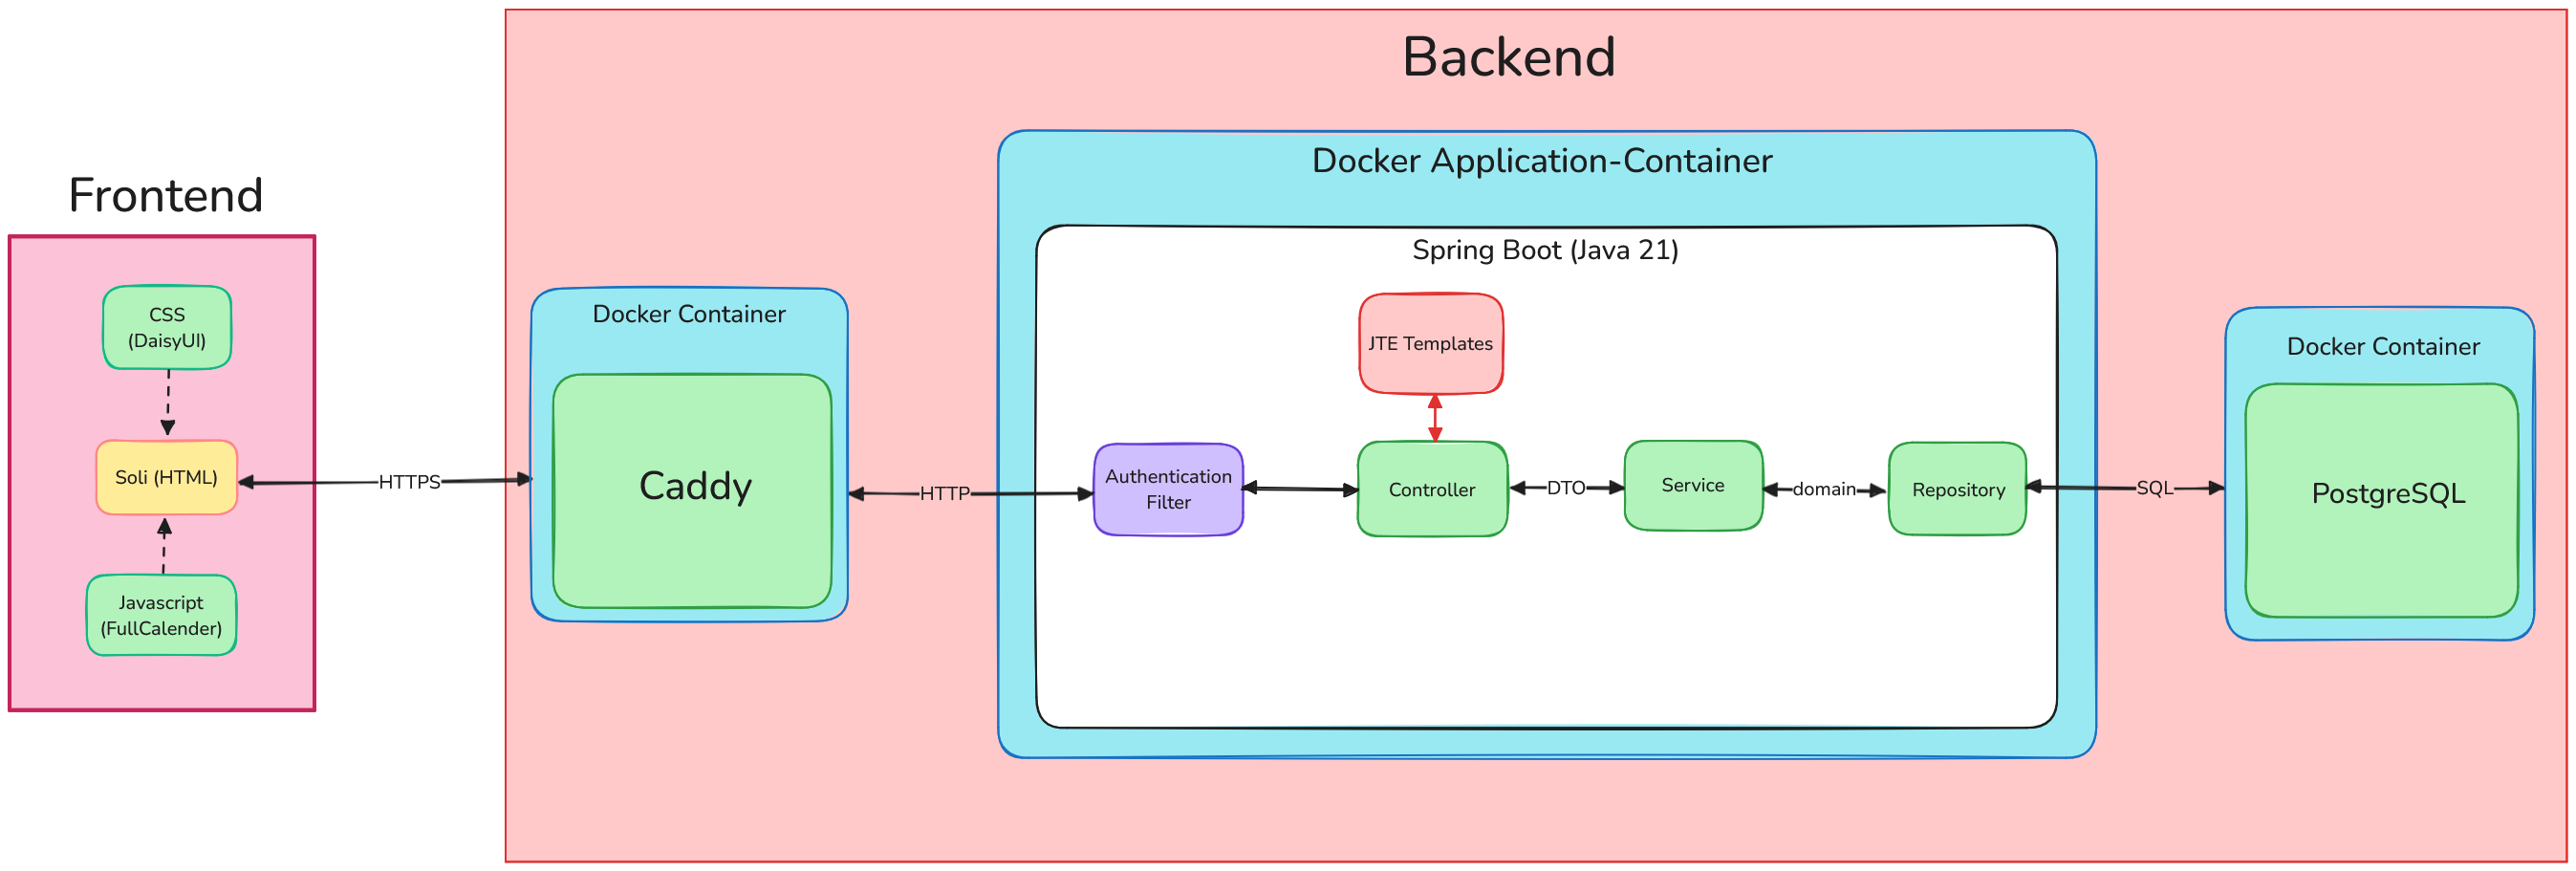
\includegraphics[width=\textwidth]{figures/architecture}
    \label{fig:architekturmodell}
\end{figure}
Die Architektur ist in \textbf{Frontend} und \textbf{Backend} unterteilt und folgt der \textbf{MVC-Struktur} zur klaren Trennung der Verantwortlichkeitsbereiche.
Das \textbf{Frontend} nutzt \textbf{HTML (Soli)}, \textbf{DaisyUI} für das Design und \textbf{FullCalendar} in JavaScript für die Kalenderfunktionalität.
Die Kommunikation mit dem Backend erfolgt sicher über \textbf{HTTPS}.

Ein \textbf{Caddy-Server}, in einem Docker-Container, dient als HTTPS-Reverse-Proxy und leitet Anfragen an das Backend weiter.
Das \textbf{Backend} basiert auf \textbf{Spring Boot} (Java 21) und läuft in einem Docker-Container. Dort prüft ein \textbf{Authentication Filter} die Anfragen,
die von \textbf{Controllern} verarbeitet werden. Mithilfe von \textbf{JTE Templates} werden dynamische HTML-Antworten generiert.
Die \textbf{Businesslogik} liegt in den \textbf{Services}, die Anfragen koordinieren und weiterleiten.
Die \textbf{Repositories} kapseln den SQL-Zugriff und ermöglichen eine saubere, abstrahierte Kommunikation mit der \textbf{PostgreSQL-Datenbank} in einem separaten Container.

Dank \textbf{Server-Side Rendering} bietet die Architektur dynamische Inhalte und hohe Skalierbarkeit. Der Einsatz gängiger Technologien wie \textbf{Docker} sorgt für einfache Bereitstellung und Wartbarkeit.
\clearpage

\section{Klassendiagramm}
\begin{figure}[ht]
    \centering
    \includegraphics[width=0.62\textwidth]{figures/classes}
    \label{fig:klassendiagramm}
\end{figure}
\clearpage
%!TEX root = ../main.tex

\chapter{View}
\label{ch:view}


\section{Haupseite und Buchung}

Die Startseite der Anwendung ist in \ref{fig:startseite} dargestellt.
Auf dieser haben Nutzende die Möglichkeit, dem Raum zu buchen oder auf andere Ansichten zu wechseln.
Das Banner in allen Ansichten zeigt den aktuellen Raumstatus an.
Insbesondere wird dadurch die Priorität des aktuellen Termins mithilfe der Farbe des Banners angezeigt.

Rechts in dieser Ansicht befindet sich ein Kalender, der die aktuelle Woche und die Termine in diesem Zeitraum anzeigt.
Die Termine sind farblich nach Priorität gekennzeichnet, weitere Informationen können durch Klicken auf den Termin eingesehen werden.
Neben dieser Möglichkeit, den Raum zu buchen, gibt es je nach Anmeldungsstatus einen Anmelde- oder Abmeldebutton und einen separaten Buchungsbutton,
für die die Verwendung des Kalenders Probleme bereitet.
Falls zur Zeit der Verwendung ein Termin des Nutzenden stattfindet, wird ein Quick-Checkout Button angezeigt,
der es ermöglicht, den Raum schnell freizugeben.
Siehe dazu auch \ref{fig:checkout}.

\begin{figure}[ht]
    \centering
    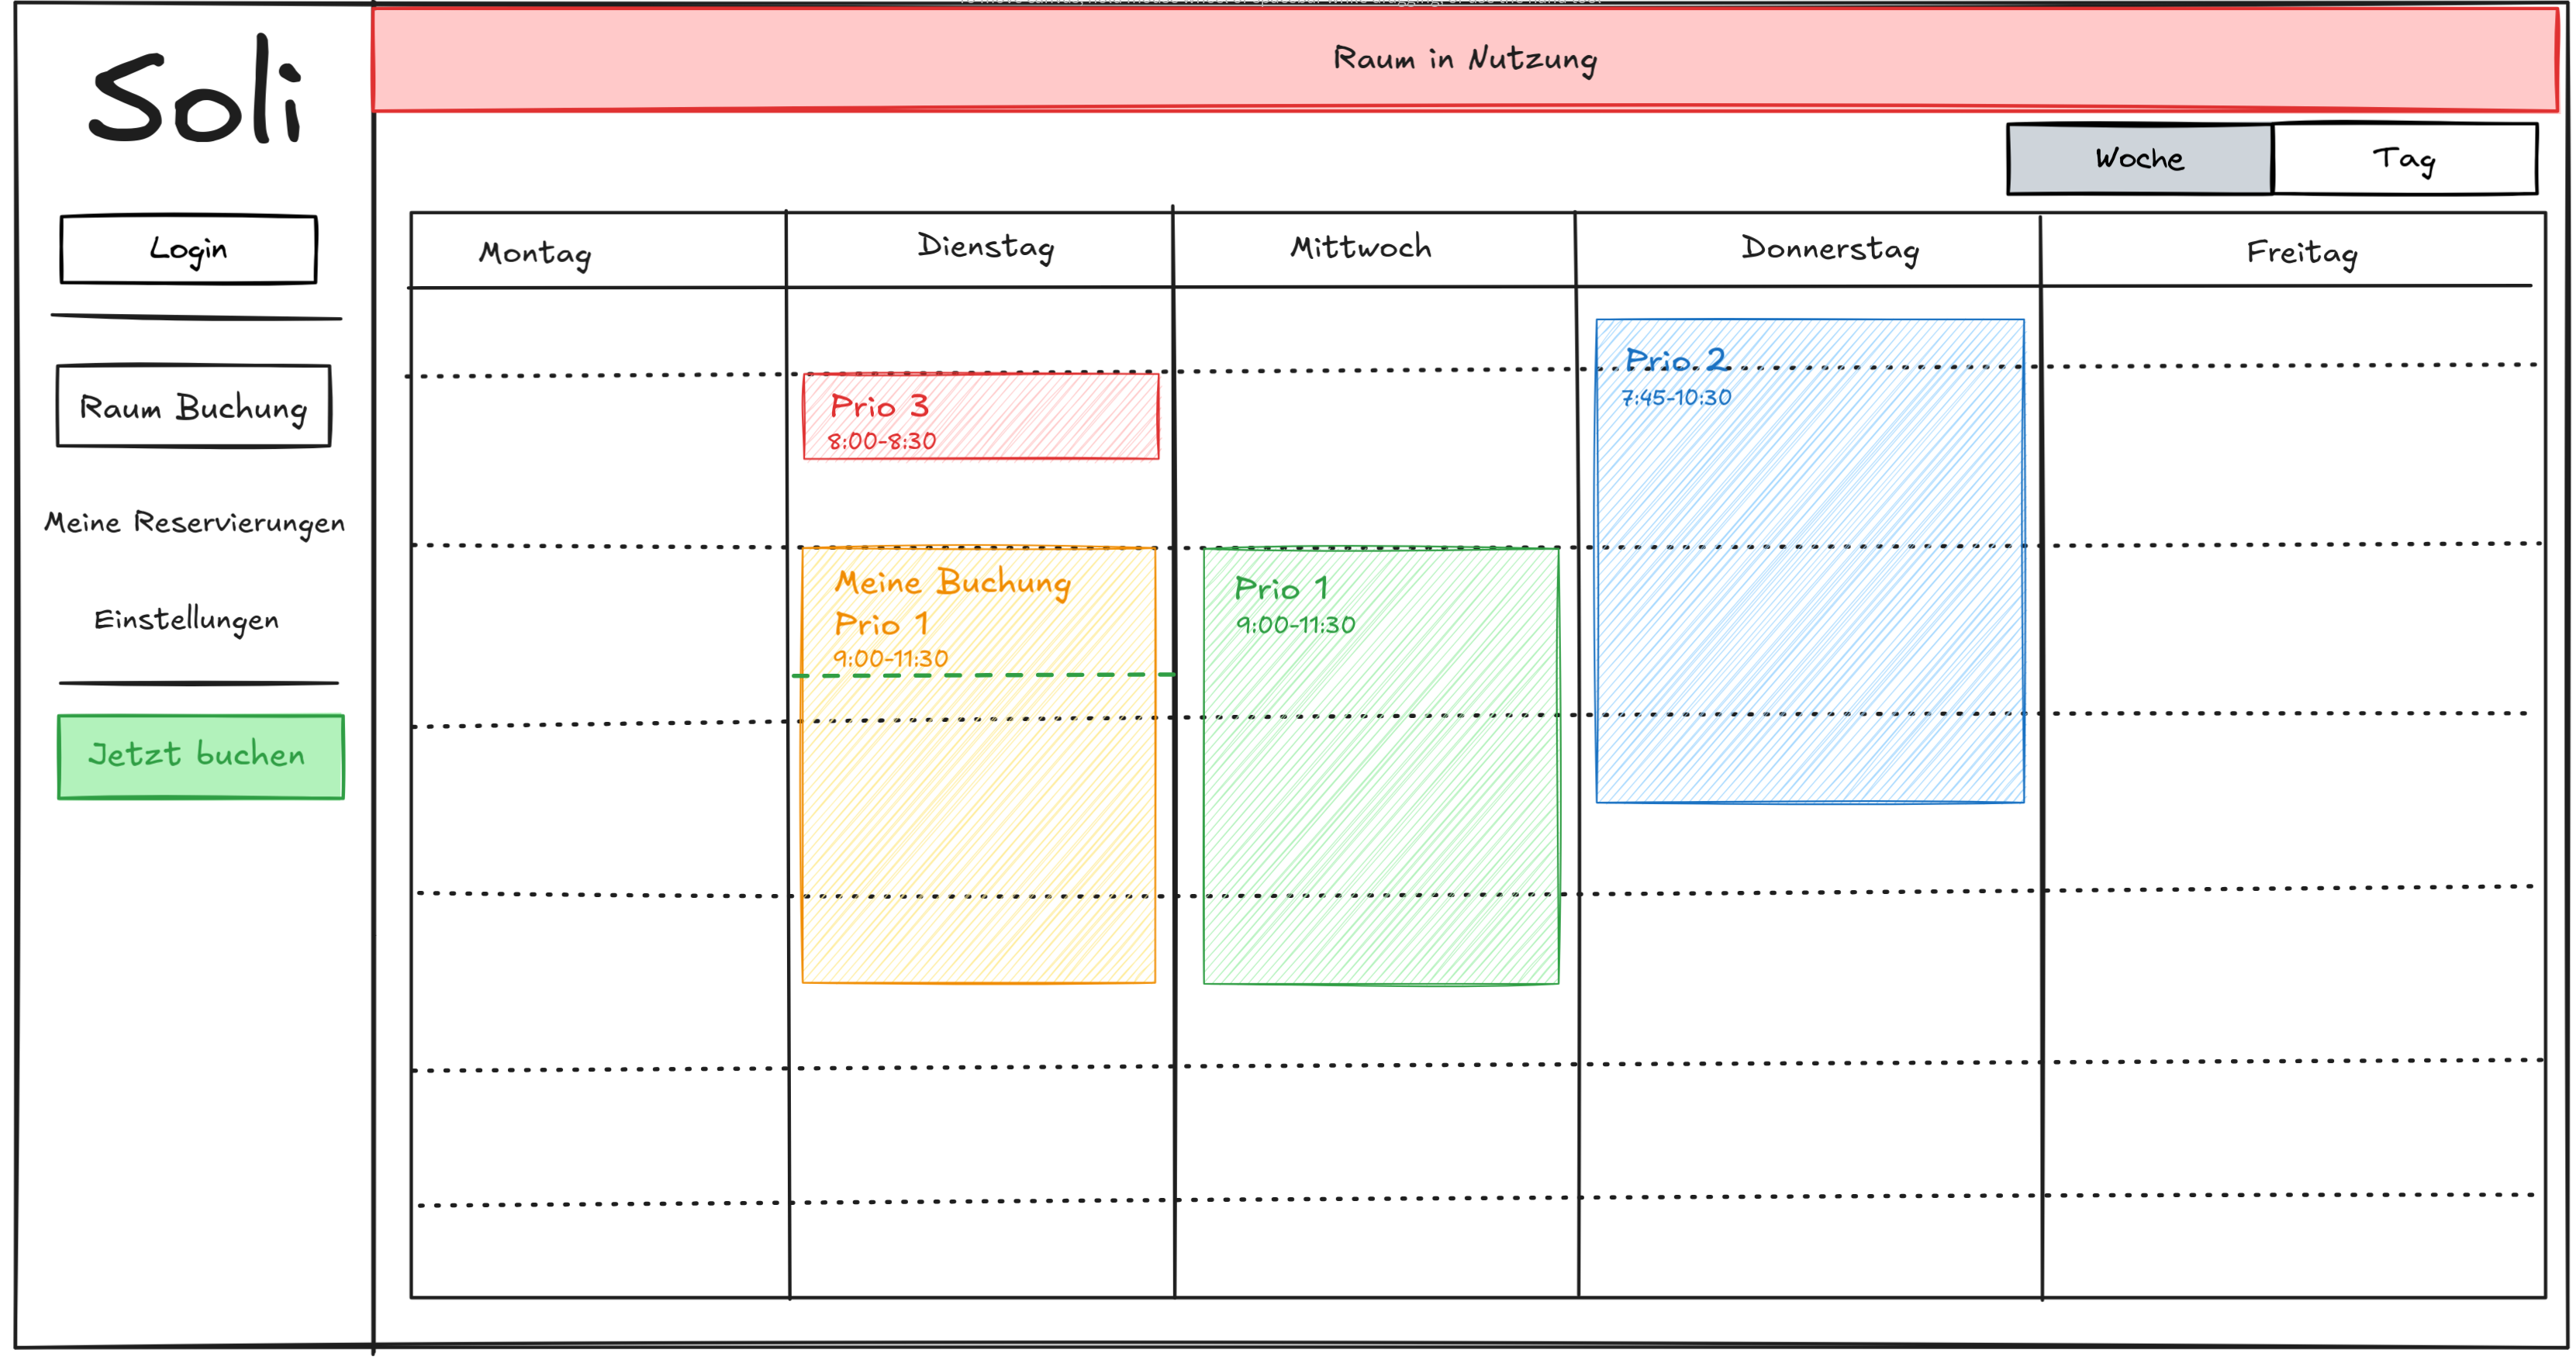
\includegraphics[width=\textwidth]{figures/ui/startseite}
    \caption{Startseite der Anwendung}
    \label{fig:startseite}
\end{figure}
\pagebreak

Sollten Nutzende eine Buchung vornehmen wollen, so klicken diese in den gewünschten Zeitraum
und es wird der Dialog in \ref{fig:buchung} dargestellt.

Der Dialog bietet Nutzenden die Möglichkeit, den genauen Start- und Endzeitpunkt des Termins festzulegen.

Außerdem können Nutzende die Priorität des Termins in Form einer Zahl zwischen 1 und 3 festlegen.
Nutzende können auch angeben, ob sie bereit sind, den Raum mit anderen Nutzenden zu teilen.
Für diesen Zweck werden ihnen drei Optionen bereitgestellt: \textit{Ja}, \textit{Nein} und \textit{Auf Anfrage}.
Siehe dazu auch \ref{fig:buchung}.

Letztlich können Nutzende eine Beschreibung für den Termin hinterlegen, die anderen angemeldeten Nutzenden angezeigt wird.

\begin{figure}[ht]
    \centering
    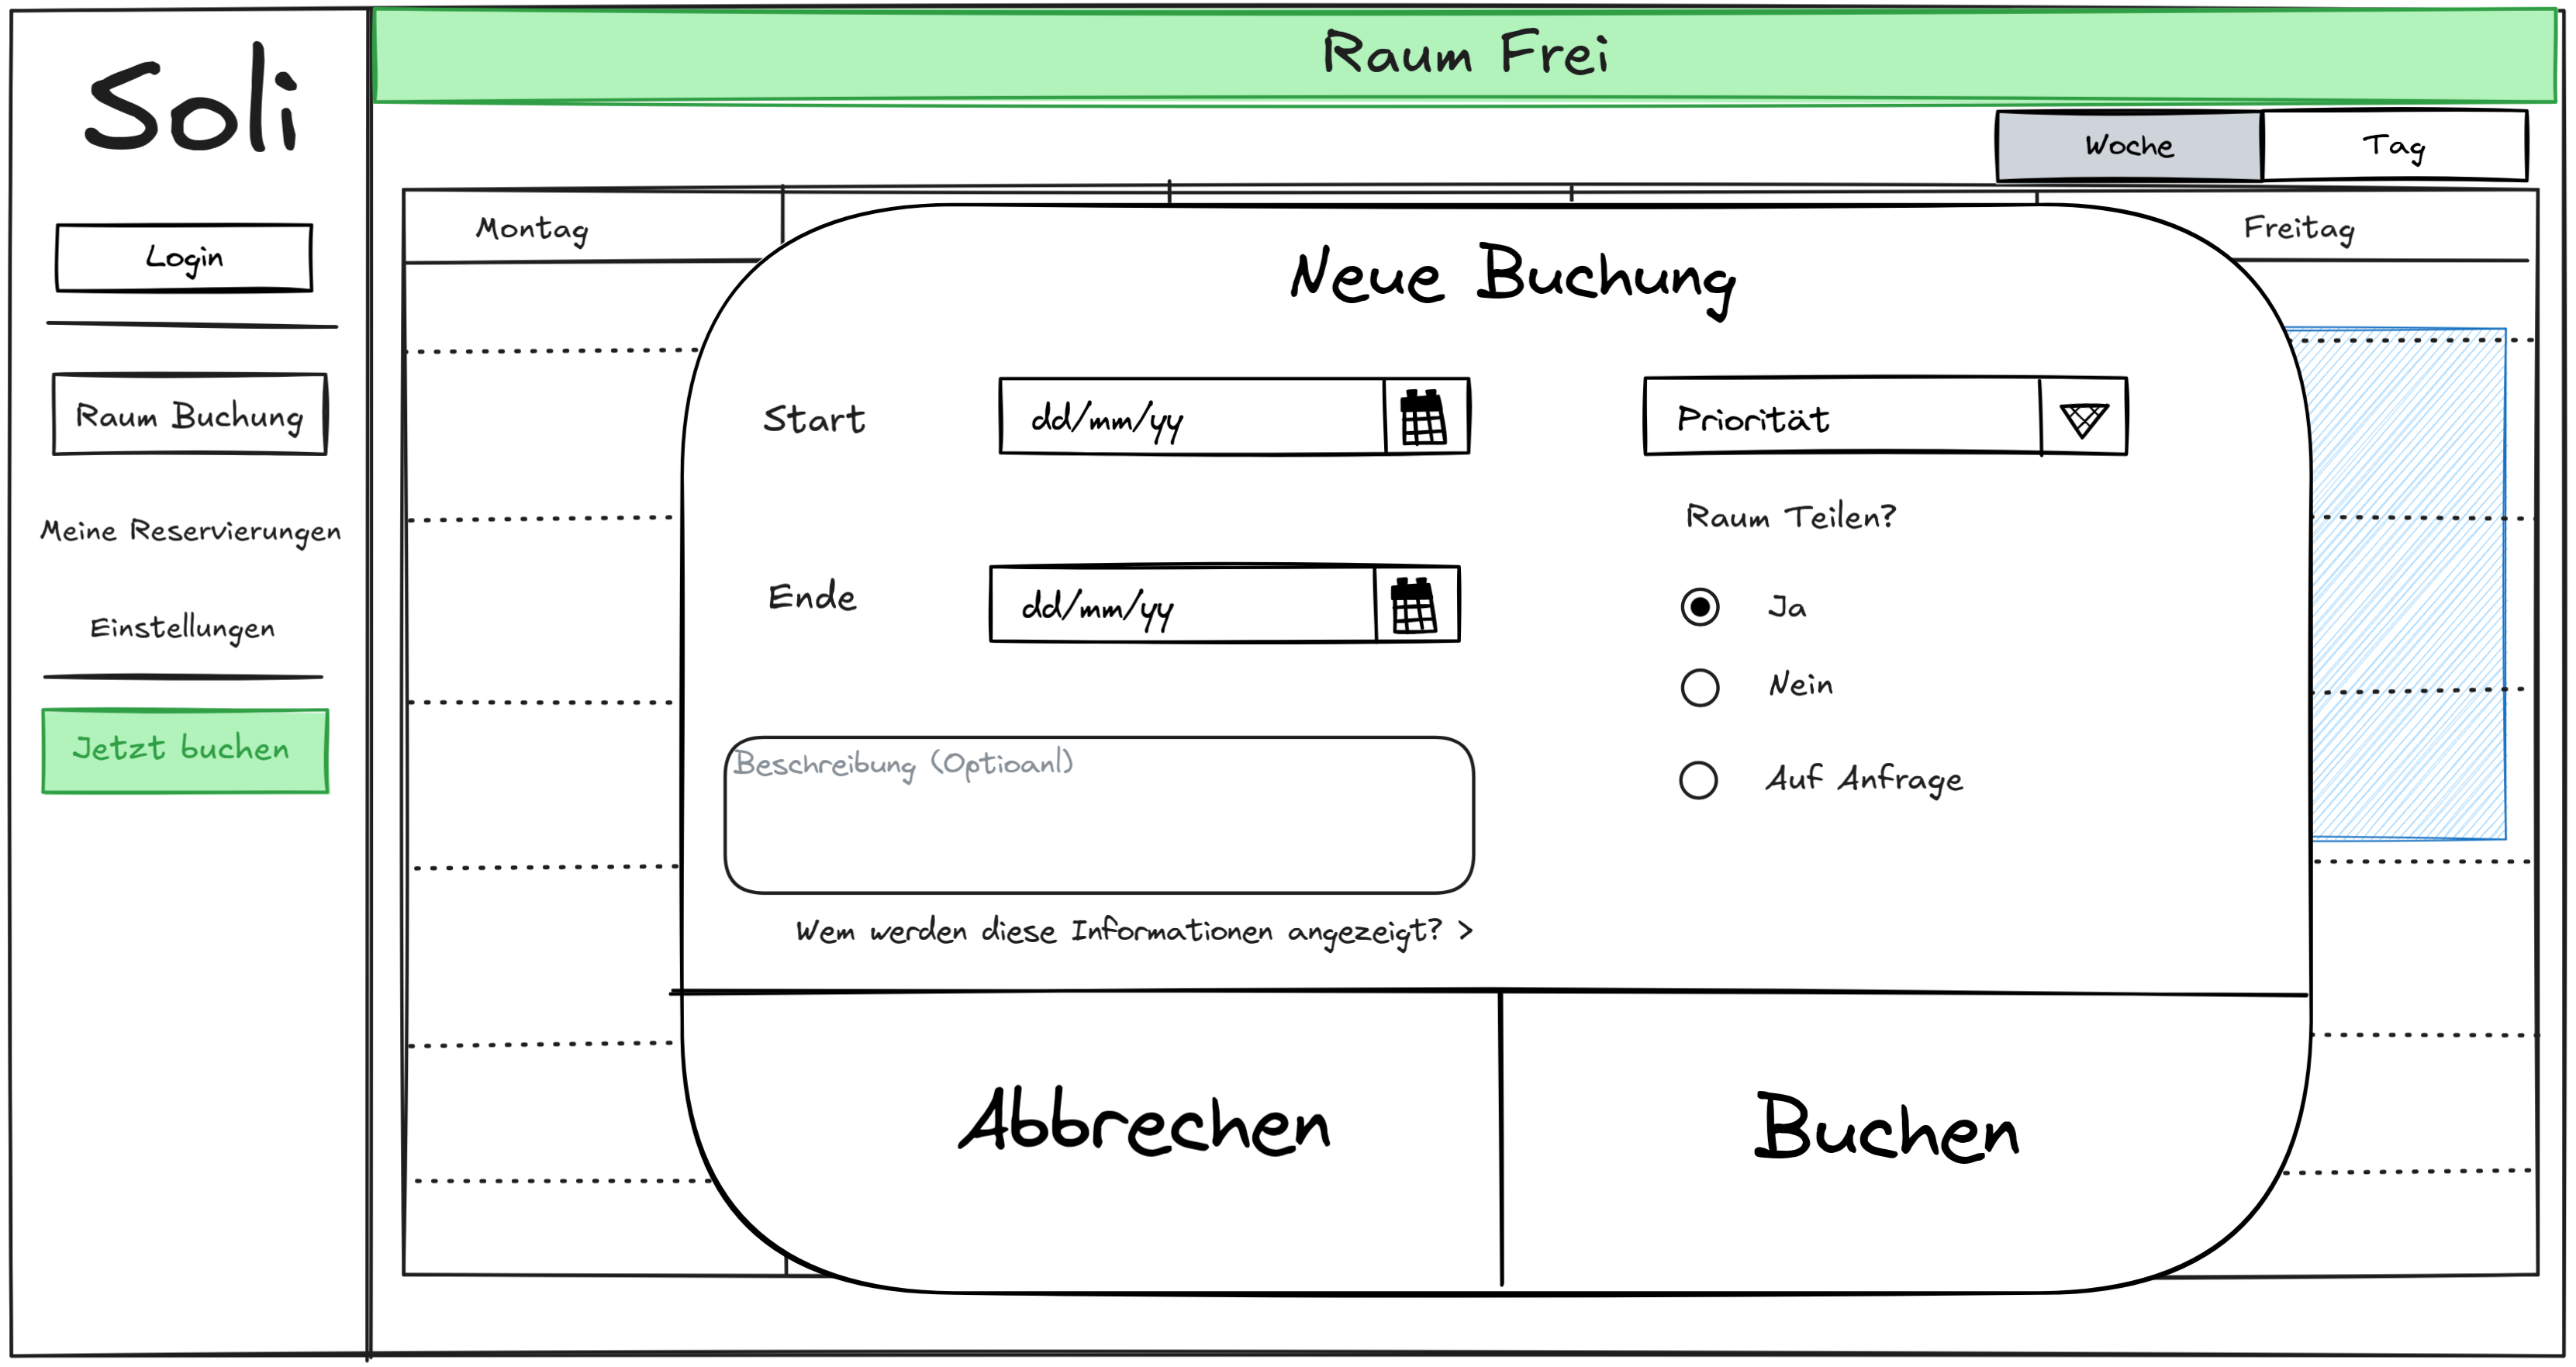
\includegraphics[width=\textwidth]{figures/ui/buchungsdialog}
    \caption{Termin-erstellen}
    \label{fig:buchung}
\end{figure}
\clearpage

Tätigen Nutzende eine Buchung, so werden diese aufgefordert, sich anzumelden.
Der hierzu gehörige Dialog ist in \ref{fig:login} dargestellt.
Alternativ ist dieser Dialog auch über den Anmeldungsbutton, der in Abbildung \ref{fig:startseite} zu sehen ist, erreichbar.

In diesem Dialog wird Nutzenden die Möglichkeit gegeben, sich mit ihrem KIT-Konto, mit einem lokalen Gastkonto oder als Admin anzumelden.

Falls Nutzende die Anmeldung per KIT-Konto wählen, werden sie auf die KIT-Login-Seite weitergeleitet.
Von dort aus können sie sich mit ihren KIT-Zugangsdaten anmelden.

Falls Nutzende die Anmeldung per Gastkonto wählen, werden sie aufgefordert, eine E-Mail-Adresse anzugeben.
Mit der Bestätigung dieser E-Mail-Adresse wird ein temporäres Gastkonto erstellt und die Anmeldung per Cookie gespeichert.

Falls Nutzende die Anmeldung als Admin wählen, werden sie aufgefordert das Passwort des Adminkontos einzugeben.

Nach einer erfolgreichen Anmeldung werden Nutzende auf die nächste Seite weitergeleitet.

\begin{figure}[ht]
    \centering
    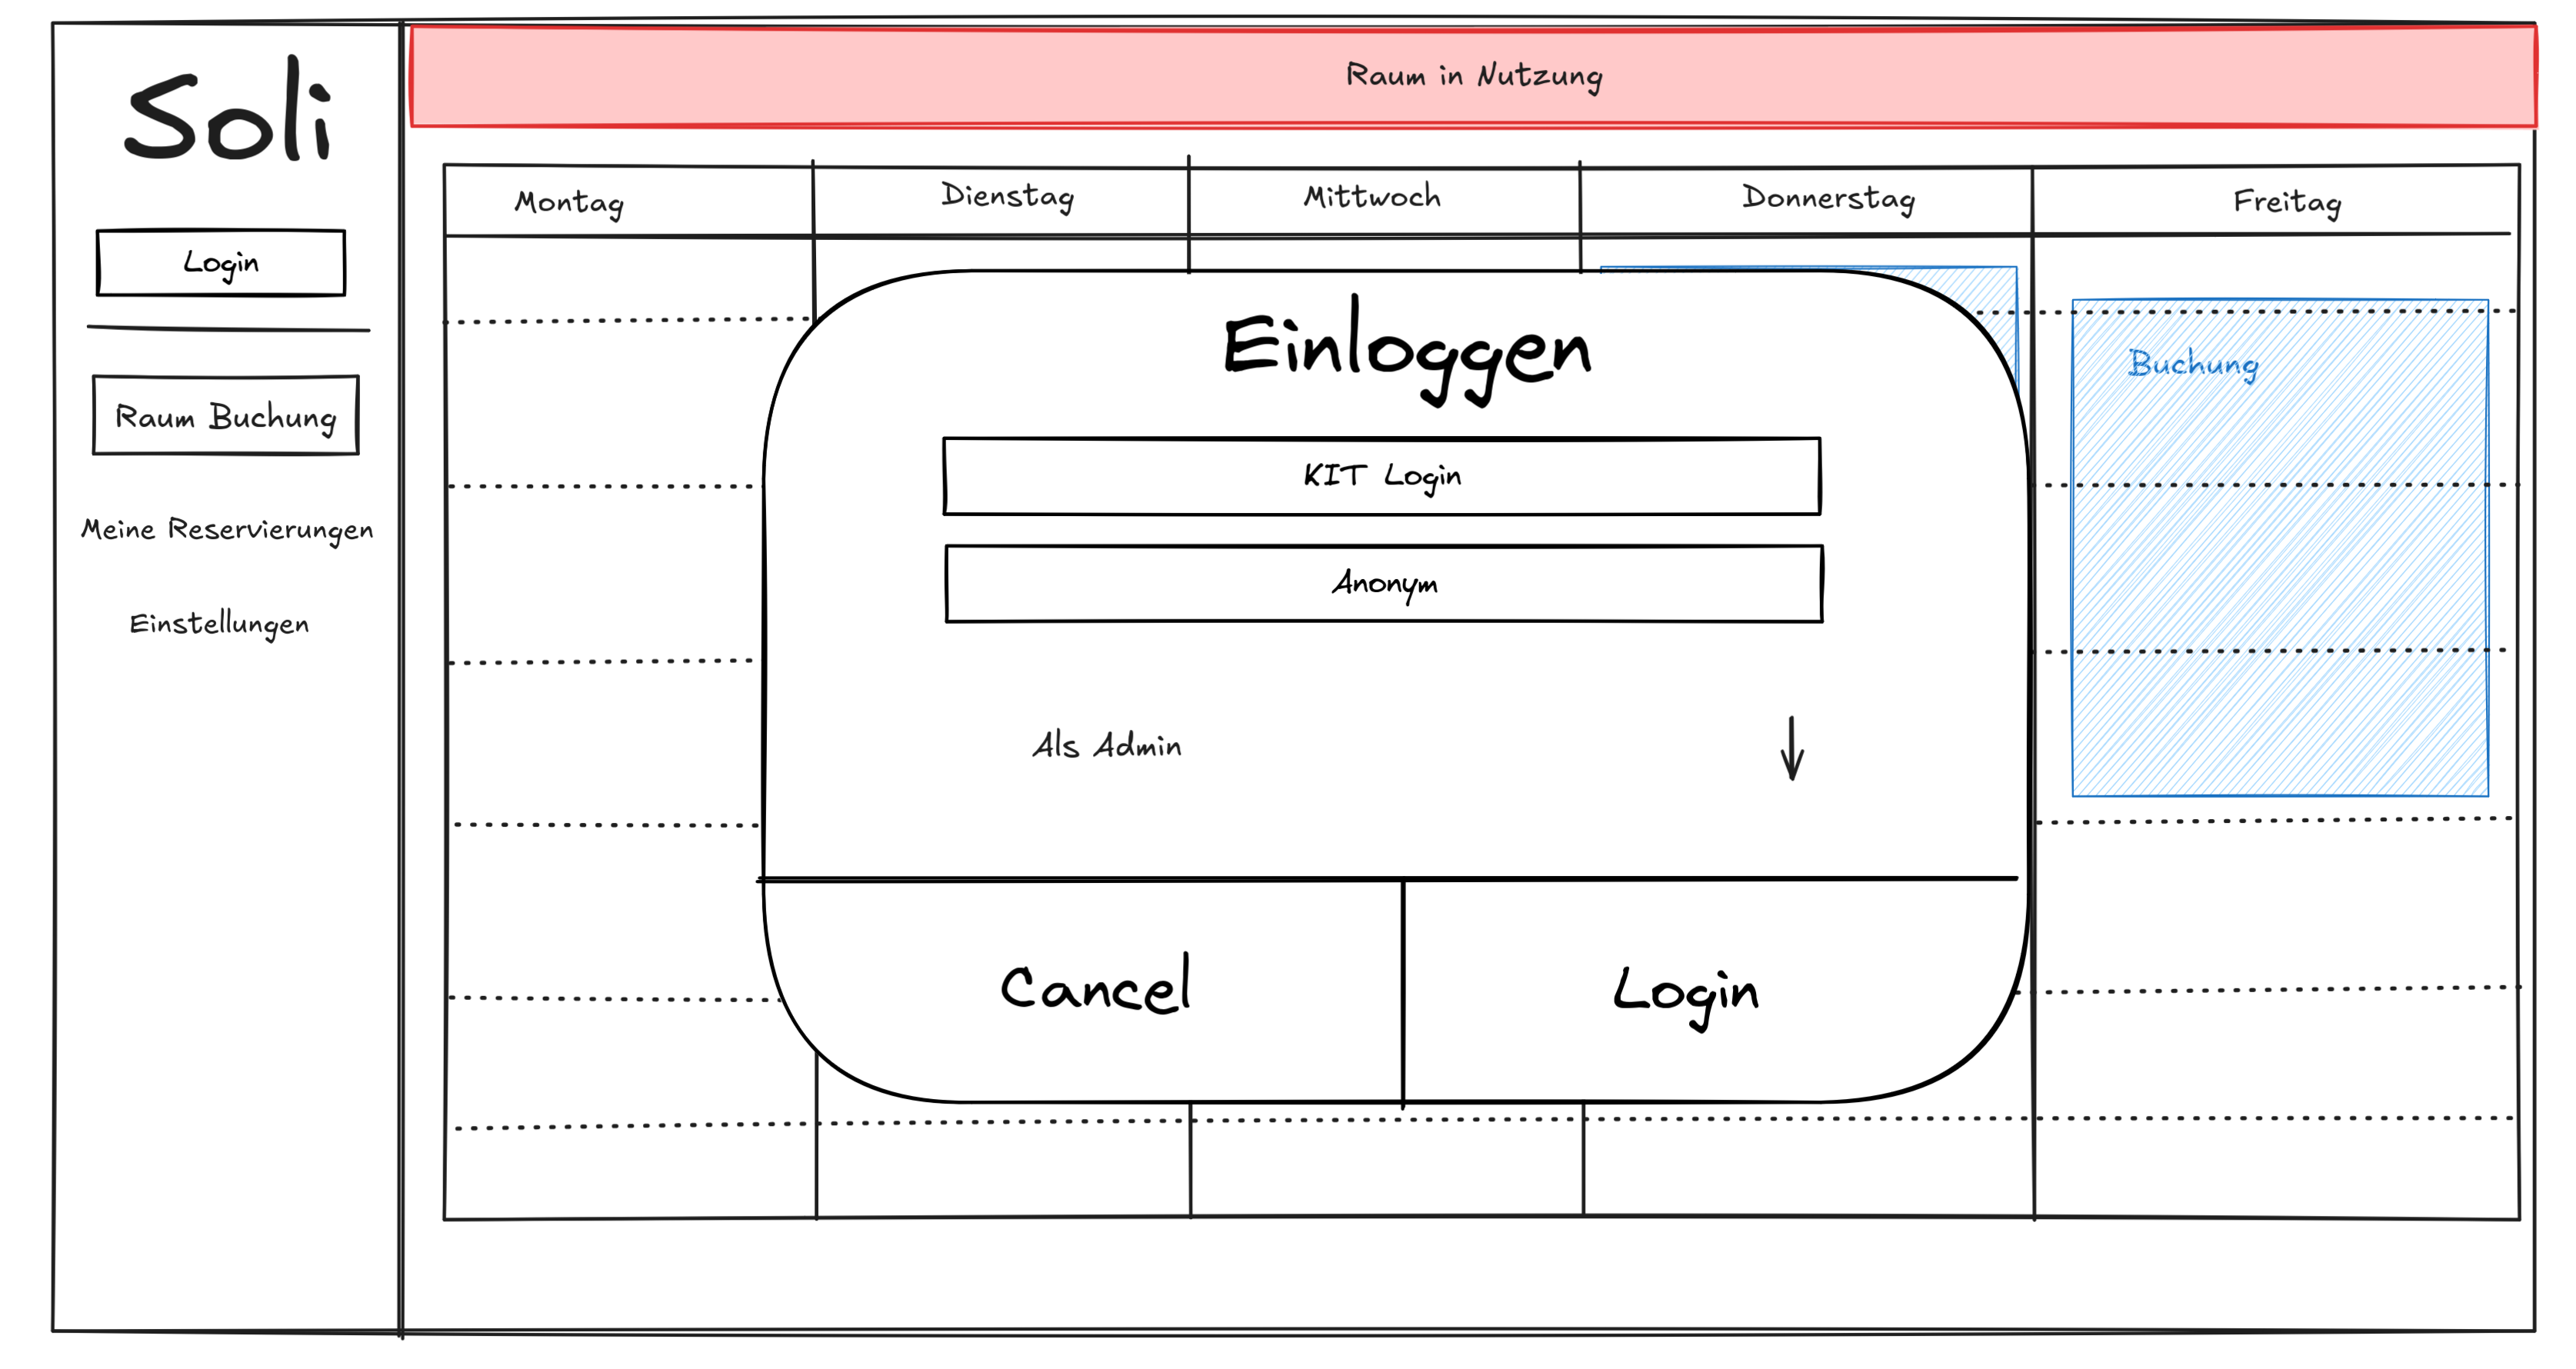
\includegraphics[width=\textwidth]{figures/ui/anmeldungsseite}
    \caption{Anmeldungsseite}
    \label{fig:login}
\end{figure}
\clearpage

Sind Nutzende eingeloggt und belegen den Raum,
so wird ihnen die in Abbildung \ref{fig:checkout} dargestellte Ansicht angezeigt.
Hier können Nutzende den Raum wieder über den Quick-Checkout Button freigeben.


Ziel dieser Ansicht ist es, Nutzenden das frühe Freigeben des Raumes ohne unnötigen Mehraufwand zu ermöglichen.
\begin{figure}[ht]
    \centering
    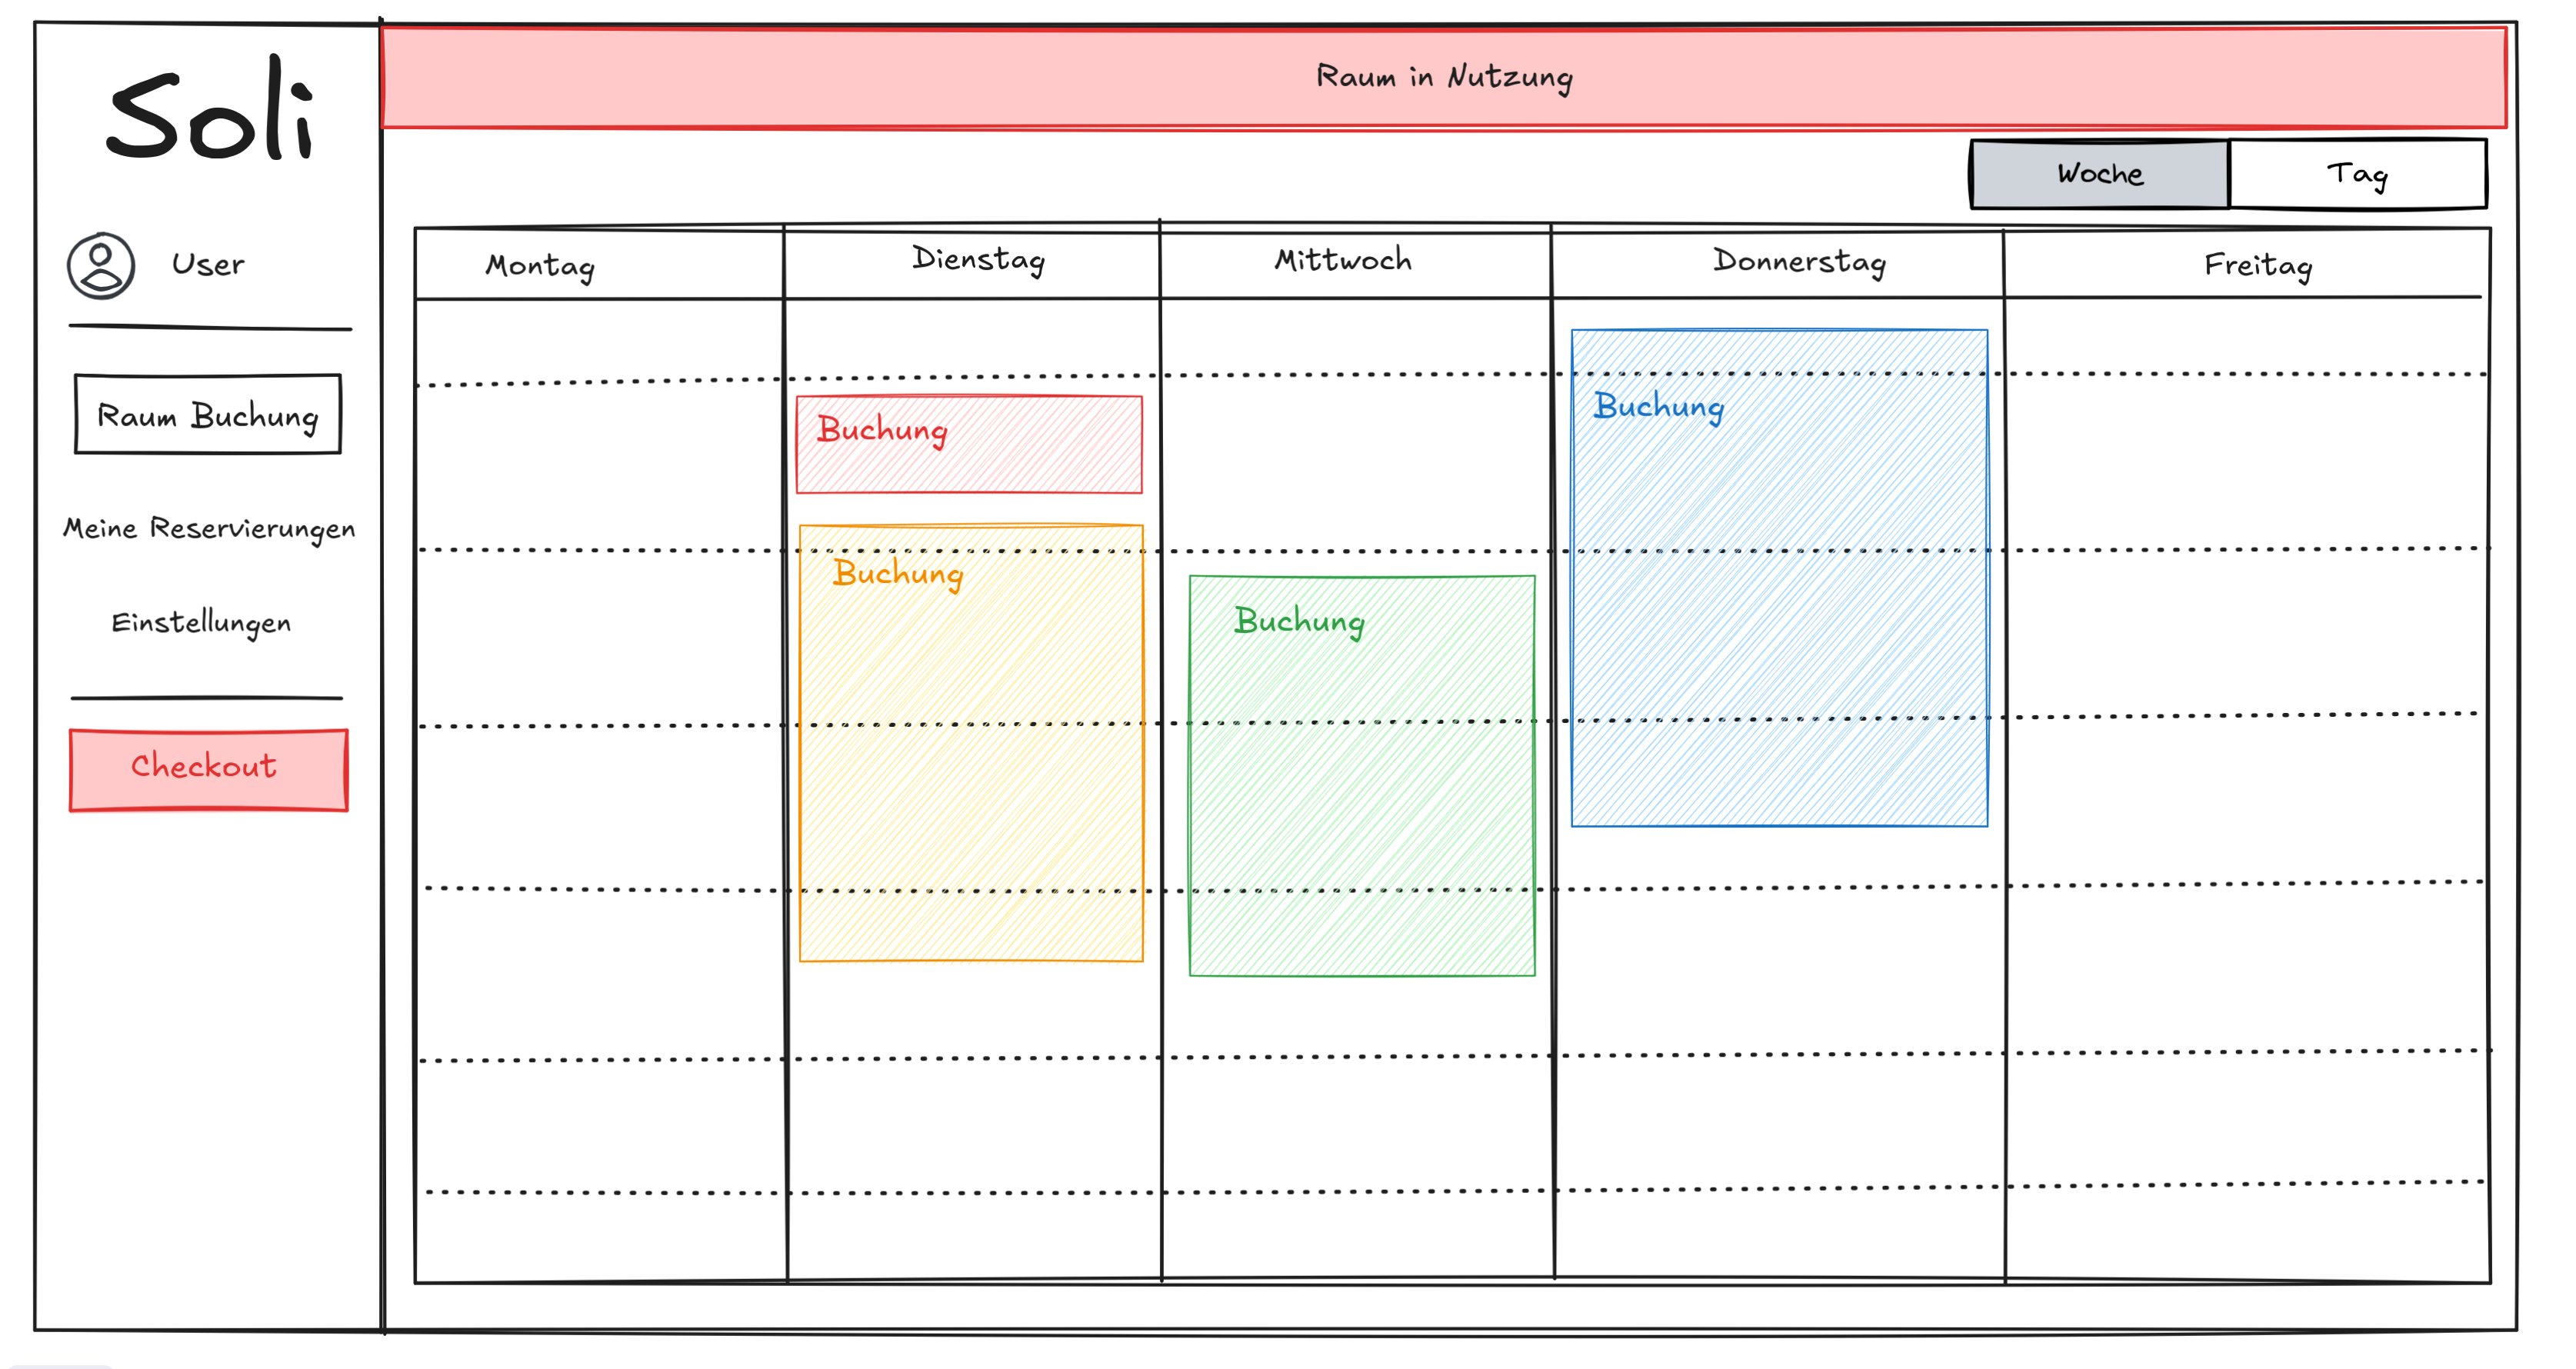
\includegraphics[width=\textwidth]{figures/ui/checkout}
    \caption{Quick Checkout}
    \label{fig:checkout}
\end{figure}
\clearpage

\section{Terminübersicht}
Nutzende, die eine Buchung vorgenommen haben, können diese in der Terminübersicht,
die in Abbildung \ref{fig:overview} dargestellt ist, einsehen und verwalten.

Die Termine in dieser Ansicht werden, anders als in der Ansicht \textit{Kalender}, in Form einer sortierten Liste dargestellt.
Dabei werden die Start- und Endzeitpunkte der Termine, wie auch die Priorität und die Beschreibung angezeigt.

Nutzende haben die Möglichkeit, eine Buchung zu stornieren, indem sie auf den Stornieren-Button klicken.

Außerdem können Nutzende die Ansicht \textit{Termin} (\ref{fig:calendarviewbooking}) zu einem Termin öffnen, indem sie auf den Termin klicken.

\begin{figure}[ht]
    \includegraphics[width=\textwidth]{figures/ui/reservierungsübersicht}
    \caption{Reservierungsübersicht}
    \label{fig:overview}
\end{figure}
\begin{figure}
    \centering
    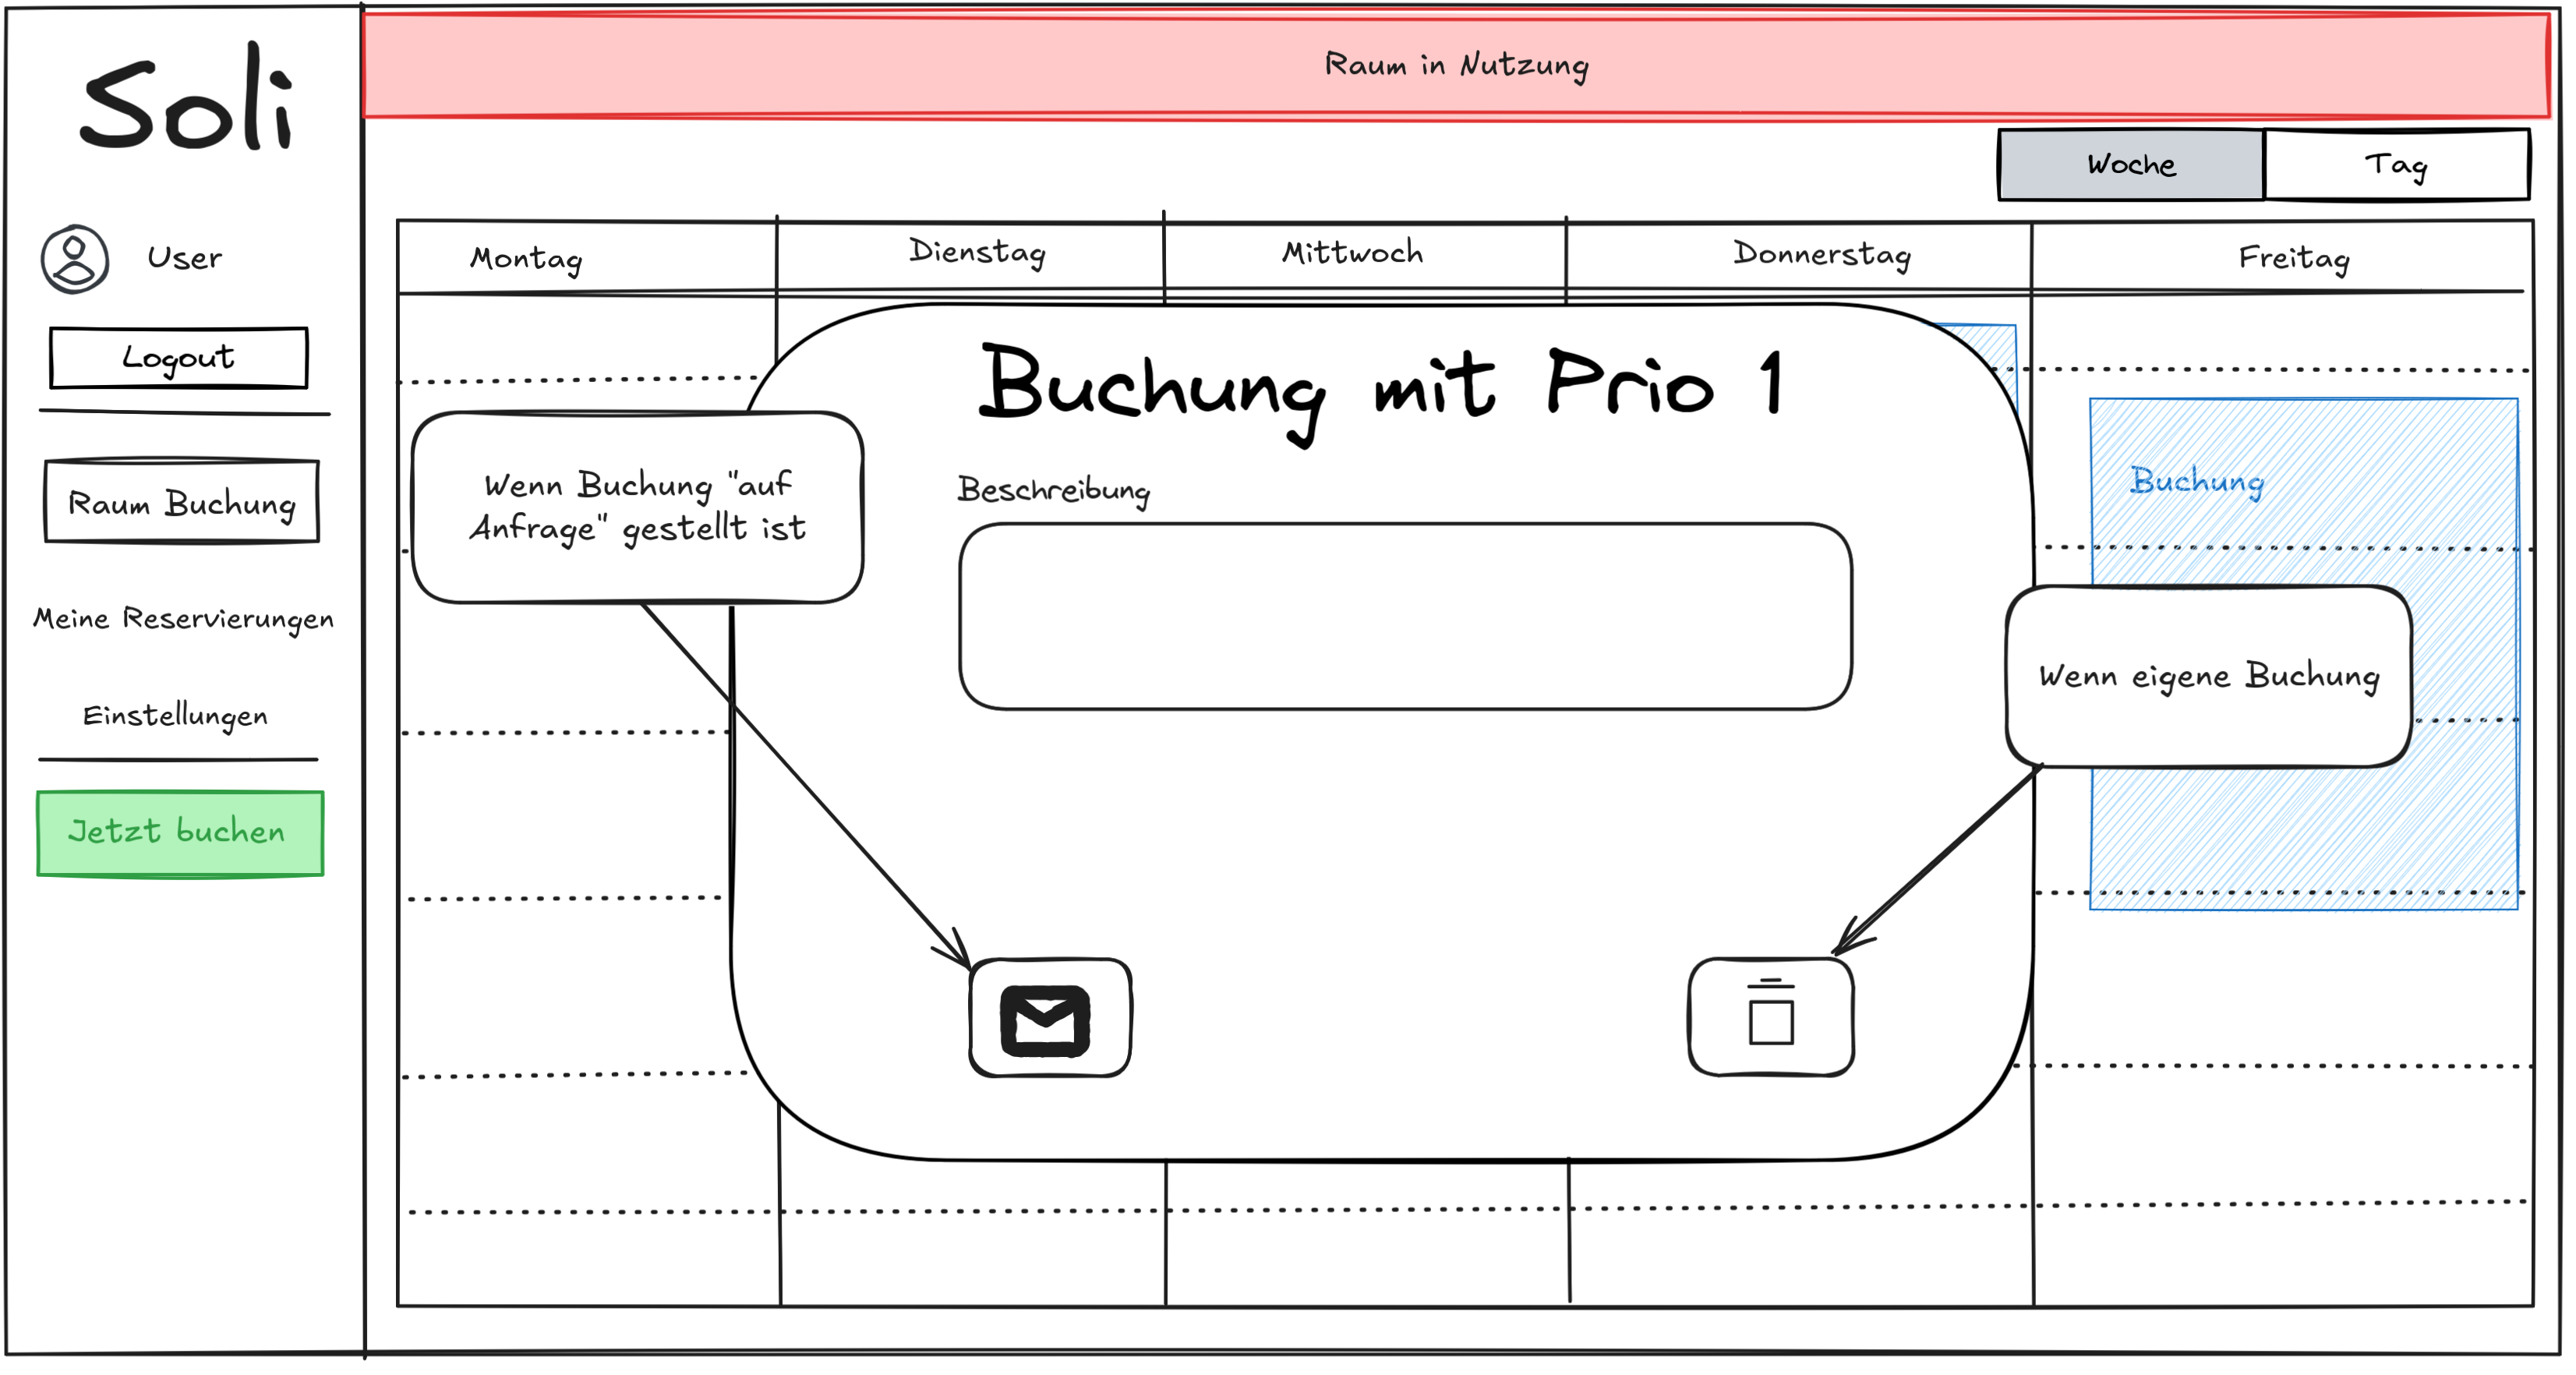
\includegraphics[width=\textwidth]{figures/ui/reservierunginkalendar}
    \caption{Reserverierung im Kalender}
    \label{fig:calendarviewbooking}
\end{figure}
\clearpage

\section{Adminstration}
Ein/e Administrator*in hat die Möglichkeit, über die Benutzeradministrationsoberfläche, die in Abbildung \ref{fig:adminuser} dargestellt ist, Nutzende einzusehen und zu verwalten.

In dieser Ansicht werden alle Nutzenden angezeigt, die sich in der Anwendung registriert haben.
Ein Admin kann die Accounts von Nutzenden deaktivieren und somit ihre Anmeldung verhindern.

Um die Suche nach einem bestimmten Konten zu erleichtern, kann ein Admin nach Kontonamen filtern.

Außerdem kann ein Admin die Anmeldung per Gastkonto deaktivieren.
Zweck dieser Funktion ist es, den Missbrauch von Gastkonten z.B.\ durch Bots in vorübergehenden Zeiten zu verhindern.

\begin{figure}[ht]
    \centering
    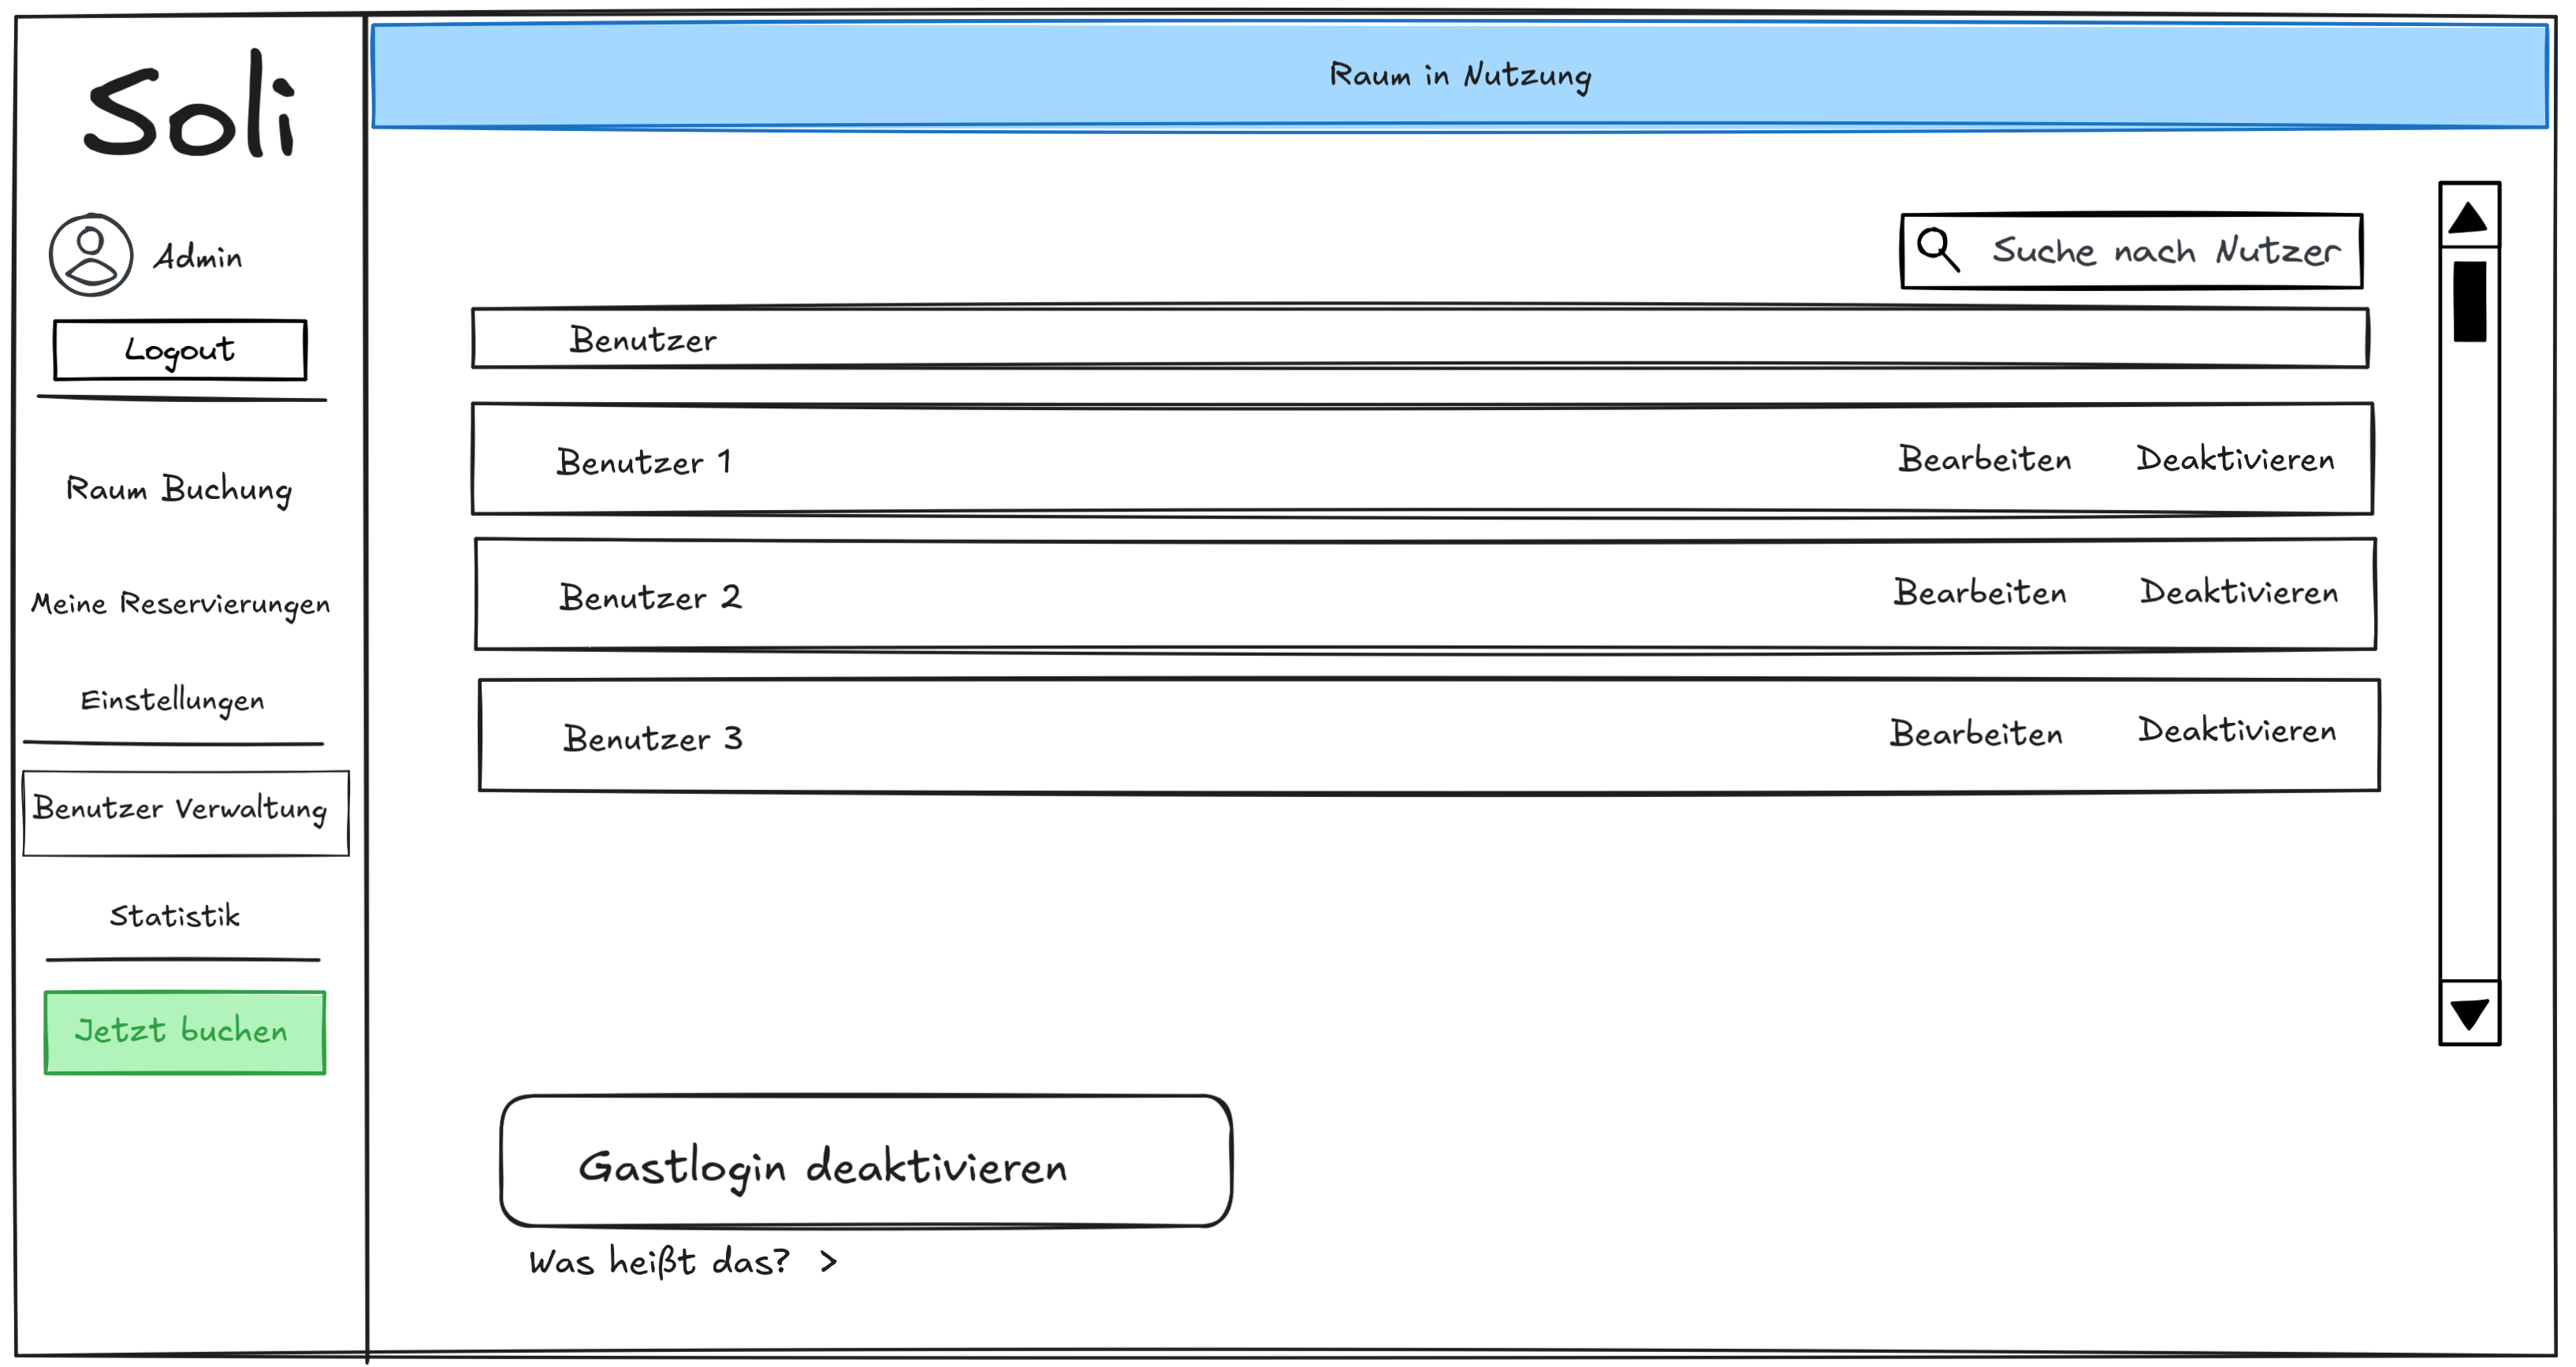
\includegraphics[width=\textwidth]{figures/ui/useradminui}
    \caption{Benutzeradminstrationsoberfläche}
    \label{fig:adminuser}
\end{figure}


%!TEX root = ../main.tex

\chapter{Controller}
\label{ch:controller}

Das Controller-Layer der Anwendung ist für die Verarbeitung von Anfragen und die Erzeugung von Antworten zuständig.
Es dekodiert und prüft dabei in \gls{HTTP}-Anfragen enthaltene Eingaben und generiert Parameter für die \gls{JTE}-Templates der View.
Zur Bearbeitung der überprüften Anfragen werden die Services des Service-Layers genutzt, welche die Datenverarbeitung kapseln.
Da einige Endpunkte eine Anmeldung benötigen, werden unangemeldete Nutzende, welche versuchen, mit einem solchen Endpunkt zu interagieren, automatisch auf die Anmeldeseite weitergeleitet.
Das Controller-Layer bietet zur Interaktion durch Nutzer die folgenden Endpunkte, welche die \gls{HTTP}-Oberfläche der Anwendung kapseln und die im Pflichtenheft beschriebenen Ansichten modellieren.

Für die Ansicht \textit{Kalender} (siehe \hyperref[edu.kit.hci.soli.controller.CalendarController]{\texttt{CalendarController}}) werden folgende Endpunkte bereitgestellt:
\begin{itemize}
    \item \texttt{GET /} gibt alle Buchungen für den Standardraum mit der fixierten ID \texttt{1} zurück.
    \item \texttt{GET /\{roomId\}} gibt die Kalenderansicht für den Raum mit der ID \texttt{roomId} zurück.
          Als Implementation für den Kalender wird dabei \gls{FullCalendar} genutzt.
    \item \texttt{GET /api/\{roomId\}/events} gibt alle Buchungen für einen Raum im \gls{FullCalendar}-Format zurück.
          Dieser Endpunkt wird von \gls{FullCalendar} genutzt, um die Buchungen im Kalender anzuzeigen.
          Links zur Ansicht \texttt{Termin} werden für die Termine eingebettet.
          Da es sich bei diesem Endpunkt um einen \gls{REST}-Endpunkt handelt, ist er separat in \hyperref[edu.kit.hci.soli.controller.EventFeedController]{\texttt{EventFeedController}} implementiert.
\end{itemize}

Für die Ansichten \textit{Termin} und \textit{Terminübersicht} (siehe \hyperref[edu.kit.hci.soli.controller.BookingViewController]{\texttt{BookingViewController}}) werden folgende Endpunkte bereitgestellt:
\begin{itemize}
    \item \texttt{GET /\{roomId\}/bookings} gibt die Terminübersicht des angemeldeten Nutzers für den Raum mit der ID \texttt{roomId} zurück.
    \item \texttt{GET /\{roomId\}/bookings/\{eventId\}} gibt die Ansicht \textit{Termin} für den Termin \texttt{eventId} zurück.
          Falls ein Administrator oder die Person, welche den Termin erstellte, angemeldet ist, wird eine Option, den Termin zu löschen, als Link eingebettet.
          Falls der Termin als kollaborativ markiert ist, wird ein link zur Ansicht \textit{Termin-Erstellen} mit den Start- und Endzeiten des angewählten Termins eingebettet.
    \item \texttt{DELETE /\{roomId\}/bookings/\{eventId\}} löscht den Termin \texttt{eventId} und leitet Nutzende auf die Terminübersicht weiter.
\end{itemize}

Für die Ansicht \textit{Termin-Erstellen} (siehe \hyperref[edu.kit.hci.soli.controller.BookingCreateController]{\texttt{BookingCreateController}}) werden folgende Endpunkte bereitgestellt:
\begin{itemize}
    \item \texttt{GET /\{roomId\}/bookings/new} gibt das Formular (implementiert als \gls{HTML-Form}) zur Erstellung eines neuen Termins für den Raum mit der ID \texttt{roomId} zurück.
    \item \texttt{POST /\{roomId\}/bookings/new} erstellt einen neuen Termin für den Raum mit der ID \texttt{roomId} und leitet Nutzende auf die Ansicht \textit{Termin} weiter.
          Die Form-Eingaben des Formulars werden dabei dekodiert und geprüft.
          Falls ein Konflikt mit einem bereits bestehenden Termin besteht, werden Nutzende auf die Konfliktseite weitergeleitet.
          In diesem Fall wird der dekodierte Termin als \hyperref[edu.kit.hci.soli.domain.Booking]{\texttt{Booking}} in der Session gespeichert.
    \item \texttt{POST /\{roomId\}/bookings/new/conflict} bietet Nutzenden die Möglichkeit, einen Konflikt entsprechend der Spezifikation im Pflichtenheft zu lösen.
          Dabei wird eine mögliche Lösung vorgeschlagen, welche Nutzende bestätigen oder ablehnen können.
          Im Falle der Bestätigung wird der in der Session gespeicherte Termin erstellt und Nutzende auf die Ansicht \textit{Termin} weitergeleitet.
          War unter den Konflikten ein Termin, welcher Zustimmung zur Kollaboration benötigt, wird entsprechend eine E-Mail an die betroffenen Nutzenden versendet.
          War unter den Konflikten ein Termin, welcher durch die Erstellung gelöscht wurde, wird entsprechend eine E-Mail an die betroffenen Nutzenden versendet.
\end{itemize}

Für die Ansicht \textit{Login} (siehe \hyperref[edu.kit.hci.soli.controller.LoginController]{\texttt{LoginController}}) werden folgende Endpunkte bereitgestellt:
\begin{itemize}
    \item \texttt{GET /login} gibt das Formular zur Anmeldung zurück. Die Anmeldung kann mit einem eingebetteten Formular als Administrator oder mit einem Link als Gast oder über \gls{OIDC} erfolgen.
          Für die Anmeldung als Administrator wird eine \gls{HTML-Form} genutzt, welche die Eingabe eines Passworts fordert.
    \item \texttt{POST /login} erlaubt die Anmeldung mit lokalen Anmeldedaten (also als Gast oder Administrator) und leitet Nutzende auf die Ansicht, welche die Anmeldung verursachte, oder die Ansicht \textit{Kalender} weiter.
          Dieser Endpunkt wird bei Bestätigung einer Gast- oder Administratoren-Anmeldung aufgerufen.
    \item \texttt{GET /login/guest} gibt das Formular zur Anmeldung als Gast zurück.
    \item \texttt{GET /oauth2/authorization/kit} verarbeitet die Anmeldung über \gls{OIDC} und leitet Nutzende auf die Ansicht, welche die Anmeldung verursachte, oder die Ansicht \textit{Kalender} weiter.
          Auf diesen Endpunkt werden Nutzende bei Bestätigung einer \gls{OIDC}-Anmeldung durch den OIDC-Server weitergeleitet.
\end{itemize}

Für die Ansicht \textit{Kontoliste} (siehe \hyperref[edu.kit.hci.soli.controller.UsersController]{\texttt{UsersController}}) werden folgende Endpunkte bereitgestellt:
\begin{itemize}
    \item \texttt{GET /admin/users} gibt die Kontoliste aller Nutzenden zurück. Das Administrationskonto wird dabei nicht angezeigt.
          Für jedes Konto wird ein Link zur Deaktivierung als \gls{HTML-Form} eingebettet (dies erlaubt die Nutzung von \texttt{PUT}-Anfragen).
    \item \texttt{GET /admin/users/{userId}/deactivate} gibt das Formular zur Deaktivierung des Kontos mit der ID \texttt{userId} zurück.
    \item \texttt{PUT /admin/users/{userId}/deactivate} deaktiviert das Konto mit der ID \texttt{userId} und leitet Nutzende auf die Kontoliste weiter.
    \item \texttt{PUT /admin/users/{userId}/reactivate} reaktiviert das Konto mit der ID \texttt{userId} und leitet Nutzende auf die Kontoliste weiter.
    \item \texttt{GET /admin/users/disable-guests} gibt das Formular zur Deaktivierung der Anmeldung als Gast zurück.
    \item \texttt{PUT /admin/users/disable-guests} deaktiviert den Login durch Gastkonten und leitet Nutzende auf die Kontoliste weiter.
          Zudem werden alle Buchungen von Gastkonten gelöscht.
    \item \texttt{PUT /admin/users/enable-guests} reaktiviert den Login durch Gastkonten und leitet Nutzende auf die Kontoliste weiter.
\end{itemize}

Außerdem werden folgende allgemeine Endpunkte (siehe \hyperref[edu.kit.hci.soli.controller.MainController]{\texttt{MainController}}) bereitgestellt:
\begin{itemize}
    \item \texttt{GET /error} gibt eine Fehlerseite zurück. Dieser Endpunkt wird von Spring automatisch aufgerufen, wenn ein Fehler auftritt.
    \item \texttt{GET /disabled} gibt eine Seite zurück, die Nutzende darüber informiert, dass ihr Konto deaktiviert wurde.
\end{itemize}

\InputIfFileExists{javadoc/edu.kit.hci.soli.controller}{}{}
%!TEX root = ../main.tex

\chapter{Services}
\label{ch:services}

Der Service-Layer koordiniert die Logik der Applikation und stellt diese den Endpunkten, beispielsweise den Controllern bereit.
Somit wird auch die Datenverarbeitung von der verarbeitung der HTTP-Anfragen und antworten abgekapselt.
Zur bearbeitung dieser Aufgaben nutzen die Services den Repository-Layer, welcher die Interaktion mit der Datenbank abstrahiert.
Vor allem komplexere aufgaben, wie das Buchen eines Termines, auflösen eines Terminkonfliktes oder das
Versenden von E-Mails wird von den Services behandelt.

Der \textit{Bookings Service} beinhaltet alle Logik für das Verwalten von Terminen: Löschen, Buchen, Koordination der Raumteilung, sowie das Vorbereiten der Termine, welche in der Kalenderansicht zu beobachten sind.
Dabei wird auch ein potenziell beim Buchen entstehender Terminkonflikt identifiziert und eine mögliche Auflösung dieses Konfliktes vorbereitet.
Nachdem ein/e Nutzende*r die Auflösung des Konfliktes bestätigt hat, wird diese angewandt und die womöglich nötigen anpassungen von anderen Terminen vollzogen.

Der \textit{E-Mail Service} ermöglicht das Senden von E-Mails an die in den Konten hinterlegte E-Mail-Adresse.
Diese wurde je nach Kontotyp von den Nutzenden selber oder vom \gls{OIDC} Provider bereitgestellt.

Der \textit{Room Service} dient zur Auswahl des Raumes um welchen sich z.B. eine Buchung dreht.
Diese Klasse ermöglicht insbesondere eine einfache erweiterung der Applikation auf mehrere Räume.

Der \textit{System Configuration Service} dient zur Einstellung der Applikation bereitgestellten funktionen, so wird hier eingestellt ob Gastkonten aktiviert sind.
Wird von einem Admin die Gastkonten funktion deaktiviert, so werden von diesem Service auch die Termine aller betroffenen Konten gelöscht.

Der \textit{User Service} hilft mit dem umgang der Konten: Das Deaktivieren eines Kontos, überprüfen, ob ein Konto Admin oder Gast status besitzt und erstellen sowie Löschen von Konten.


\InputIfFileExists{javadoc/edu.kit.hci.soli.service}{}{}

%!TEX root = ../main.tex

\chapter{Daten}
\label{ch:data}

Der Daten-Layer befindet sich im Paket \hyperref[edu.kit.hci.soli.repository]{\texttt{repository}} dieses enthält Schnittstellen, die für den Datenzugriff und die Verwaltung von Entitäten in der Datenbank verantwortlich sind.
Hierfür wird das Spring Data JPA Framework verwendet, um \gls{CRUD}-Operationen und benutzerdefinierte Abfragen auf den Entitäten durchzuführen.
Die Hauptaufgaben des Daten-Layers sind:

\begin{itemize}
    \item Verwaltung von Entitäten: Es definiert Schnittstellen, die von JPA-Repository erben, um CRUD-Operationen auf den Entitäten durchzuführen.
    \item Benutzerdefinierte Abfragen: Es definiert benutzerdefinierte Abfragen, um spezifische Daten aus der Datenbank zu extrahieren.
\end{itemize}

Welche Operationen auf welcher Entität durchgeführt werden können, ist im Folgenden dargestellt.

\InputIfFileExists{javadoc/edu.kit.hci.soli.repository}{}{}

%!TEX root = ../main.tex

\chapter{Data Model}
\label{ch:data_model}

Das Data Model von \textit{Soli} ist in die Pakete \textit{dto} und \textit{domain} aufgeteilt.
Die \textit{dto}-Klassen sind die Datenübertragungsobjekte, die die Daten zwischen den Schichten des Systems übertragen.
Die \textit{domain}-Klassen sind die Datenobjekte, die in der Datenbank gespeichert werden, und bilden somit das interne Datenmodell des Systems.

Dieses Datenmodell wird mithilfe von \gls{SpringData} in der \gls{PostgreSQL}-Datenbank (welche sich zur Isolation in einem separaten \gls{Container} befindet) abgebildet.
In dieser wird das Datenmodell in Form von Tabellen und Beziehungen zwischen diesen gespeichert.
In der Anwendung werden die Datenobjekte nur im Kontext aktiver Anfragen im Arbeitsspeicher gehalten und bei Bedarf in die Datenbank geschrieben.
Als Konsequenz können die \gls{ACID}-Eigenschaften der Datenbank genutzt werden, um die Daten vor Verlust oder Inkonsistenzen zu schützen.
Damit die Daten auch über zukünftige Aktualisierungen des Systems hinweg erhalten bleiben, wird das Datenbankmigrationssystem \gls{Flyway} genutzt, der die Datenbankstruktur anpasst, wenn sich das Datenmodell ändert.

Den Kern des Buchungsmodells bildet die Klasse \hyperref[edu.kit.hci.soli.domain.Booking]{\texttt{Booking}}, die eine Buchung eines Raumes repräsentiert.
Jede Buchung ist einem Raum und einem Nutzer zugeordnet und hat einen Start- und Endzeitpunkt.
Außerdem kann eine Buchung optional einen Kommentar enthalten, der von dem Nutzer hinterlassen wurde.
Zur Umsetzung von Buchungen des Kooperationstyps \textit{ON\_REQUEST} existiert außerdem eine automatisch verwaltete Tabelle von noch offenen Anfragen für eine Buchung.

Da die Authentifikation von Nutzenden nicht durch das System selbst, sondern durch das \gls{OIDC}-System des KIT erfolgt, werden statt vollen Anmeldedaten nur die OIDC-IDs der Nutzenden gespeichert.
Diese sind im \hyperref[edu.kit.hci.soli.domain.User]{\texttt{User}}-Objekt unter dem Namen \texttt{userId} mit dem Präfix \texttt{kit/} abgelegt.
Gäste erhalten eine interne ID, welche mit dem Präfix \texttt{guest/} beginnt, und somit von den IDs der KIT-Nutzenden unterschieden werden kann.
Der Administrator des Systems hat die fixe interne ID \texttt{admin}.
Die Tabelle der Nutzenden ergänzt diese Information um die E-Mail-Adresse, den Namen, und die Sprache der Nutzenden, welche für die Kommunikation mit diesen (z.B. per E-Mail) genutzt werden.
Außerdem wird eine Flagge gespeichert, die es Administratoren ermöglicht, einzelne Nutzende zu sperren.

Eine Raumtabelle wird genutzt, um die Erweiterbarkeit des Systems zu gewährleisten.
In dieser Tabelle wird im minimalen System entsprechend der Musskriterien nur ein Raum gespeichert, welcher die ID \texttt{1} trägt.

Eine Übersicht des Datenbankmodells ist in \autoref{fig:data_model} dargestellt.

\begin{figure}[ht]
    \centering
    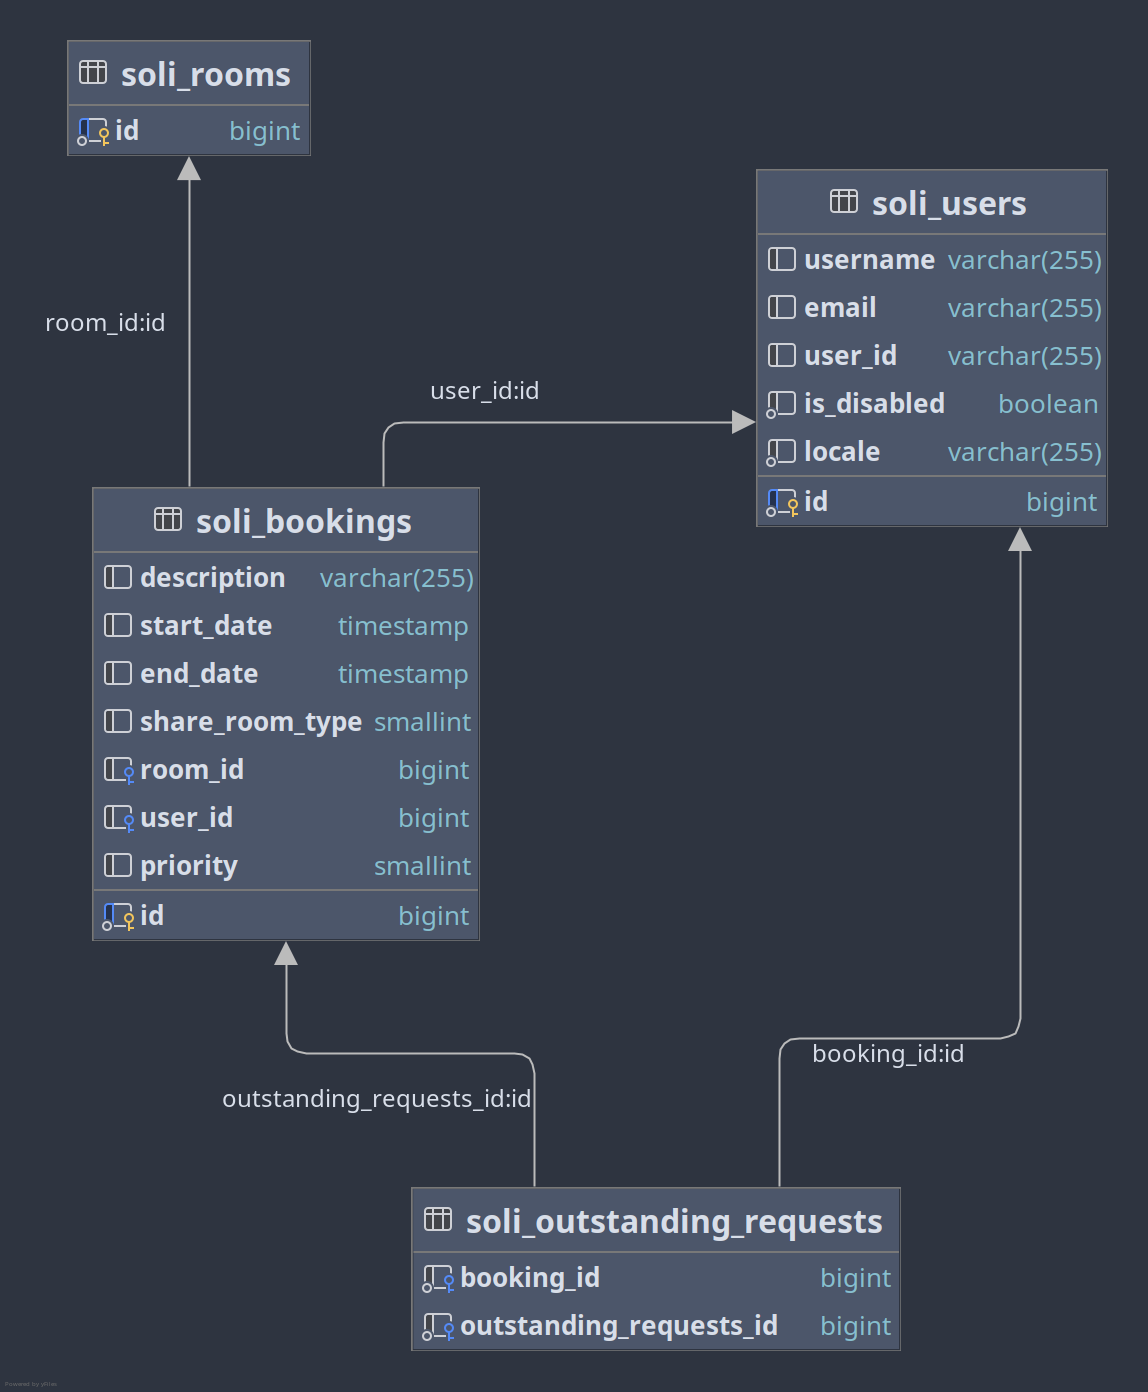
\includegraphics[width=\textwidth]{figures/database}
    \caption{Datenbankmodell von \textit{Soli}}
    \label{fig:data_model}
\end{figure}
\pagebreak

\InputIfFileExists{javadoc/edu.kit.hci.soli.dto}
\InputIfFileExists{javadoc/edu.kit.hci.soli.domain}
%!TEX root = ../main.tex

\chapter{Abläufe}
\label{ch:processes}
Im folgenden Kapitel werden die wichtigsten Abläufe des Systems beschrieben und zur Veranschaulichung in
Diagrammen dargestellt.

\section{Anmeldeprozess}
Das Programm ist so aufgebaut, dass man sich für die Interaktion mit dem System zuerst anmelden muss.
Man kann sich als Administrator*in, als Gast oder mit dem KIT-Account anmelden.

Hier wird der Ablauf des Anmeldens in einem Diagramm beschrieben.

\begin{figure}[ht]
    \centering
    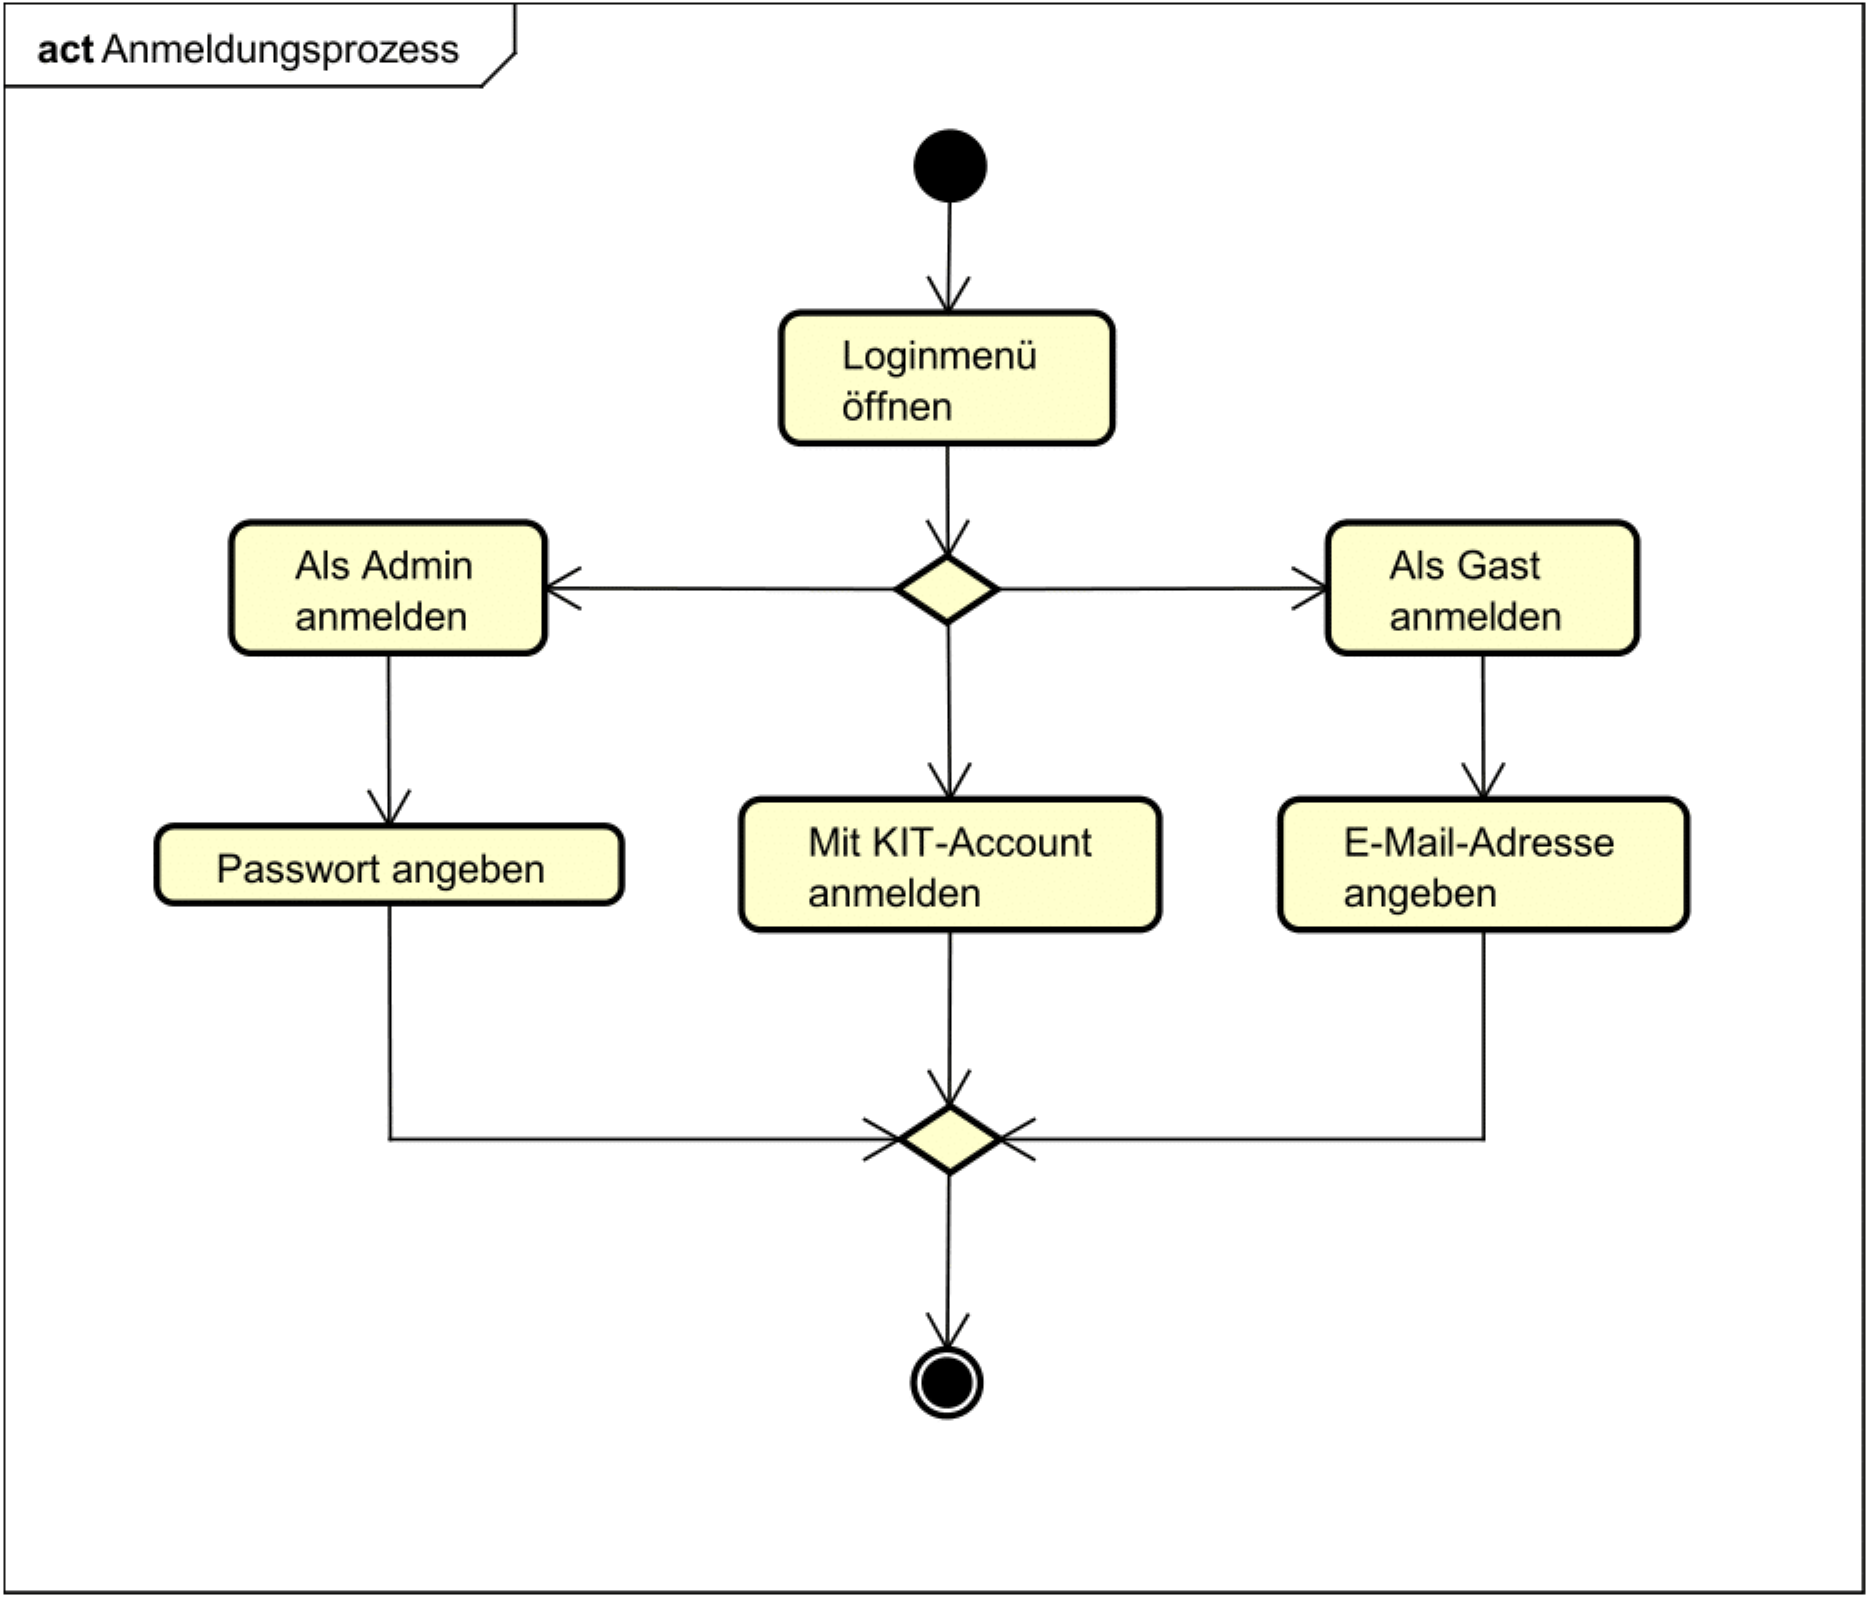
\includegraphics[width=\textwidth]{figures/activity/anmeldeprozess}
    \caption{Diagramm zur Erklärung des Anmeldeprozesses}
    \label{fig:login-diagram}
\end{figure}
\clearpage

\section{Buchung Erstellen}

\subsection{Nutzer*in erstellt Buchung}

 Weiterhin können Buchungen erstellt werden. Mit der Voraussetzung, dass die nutzende Person angemeldet ist,
kann die Buchungsansicht geöffnet werden. Dann gibt muss eine Priorität angegeben werden und festgelegt werden,
 ob man den Raum teilen möchte. Hier sind die Auswahlmöglichkeiten "Ja", "Nein" und "Auf Anfrage". Bei den "Auf
 Anfrage" gestellten Buchungen können Nuter*innen über die Website Anfragen stellen, wenn sie den Termin mit nutzen
 wollen. Weiterhin kann der ausgewählte Zeitraum angepasst oder eine Beschreibung angegeben werden.

 Das Ablaufdiagramm beschreibt den Ablauf einer Terminerstellung.

\begin{figure}[ht]
    \centering
    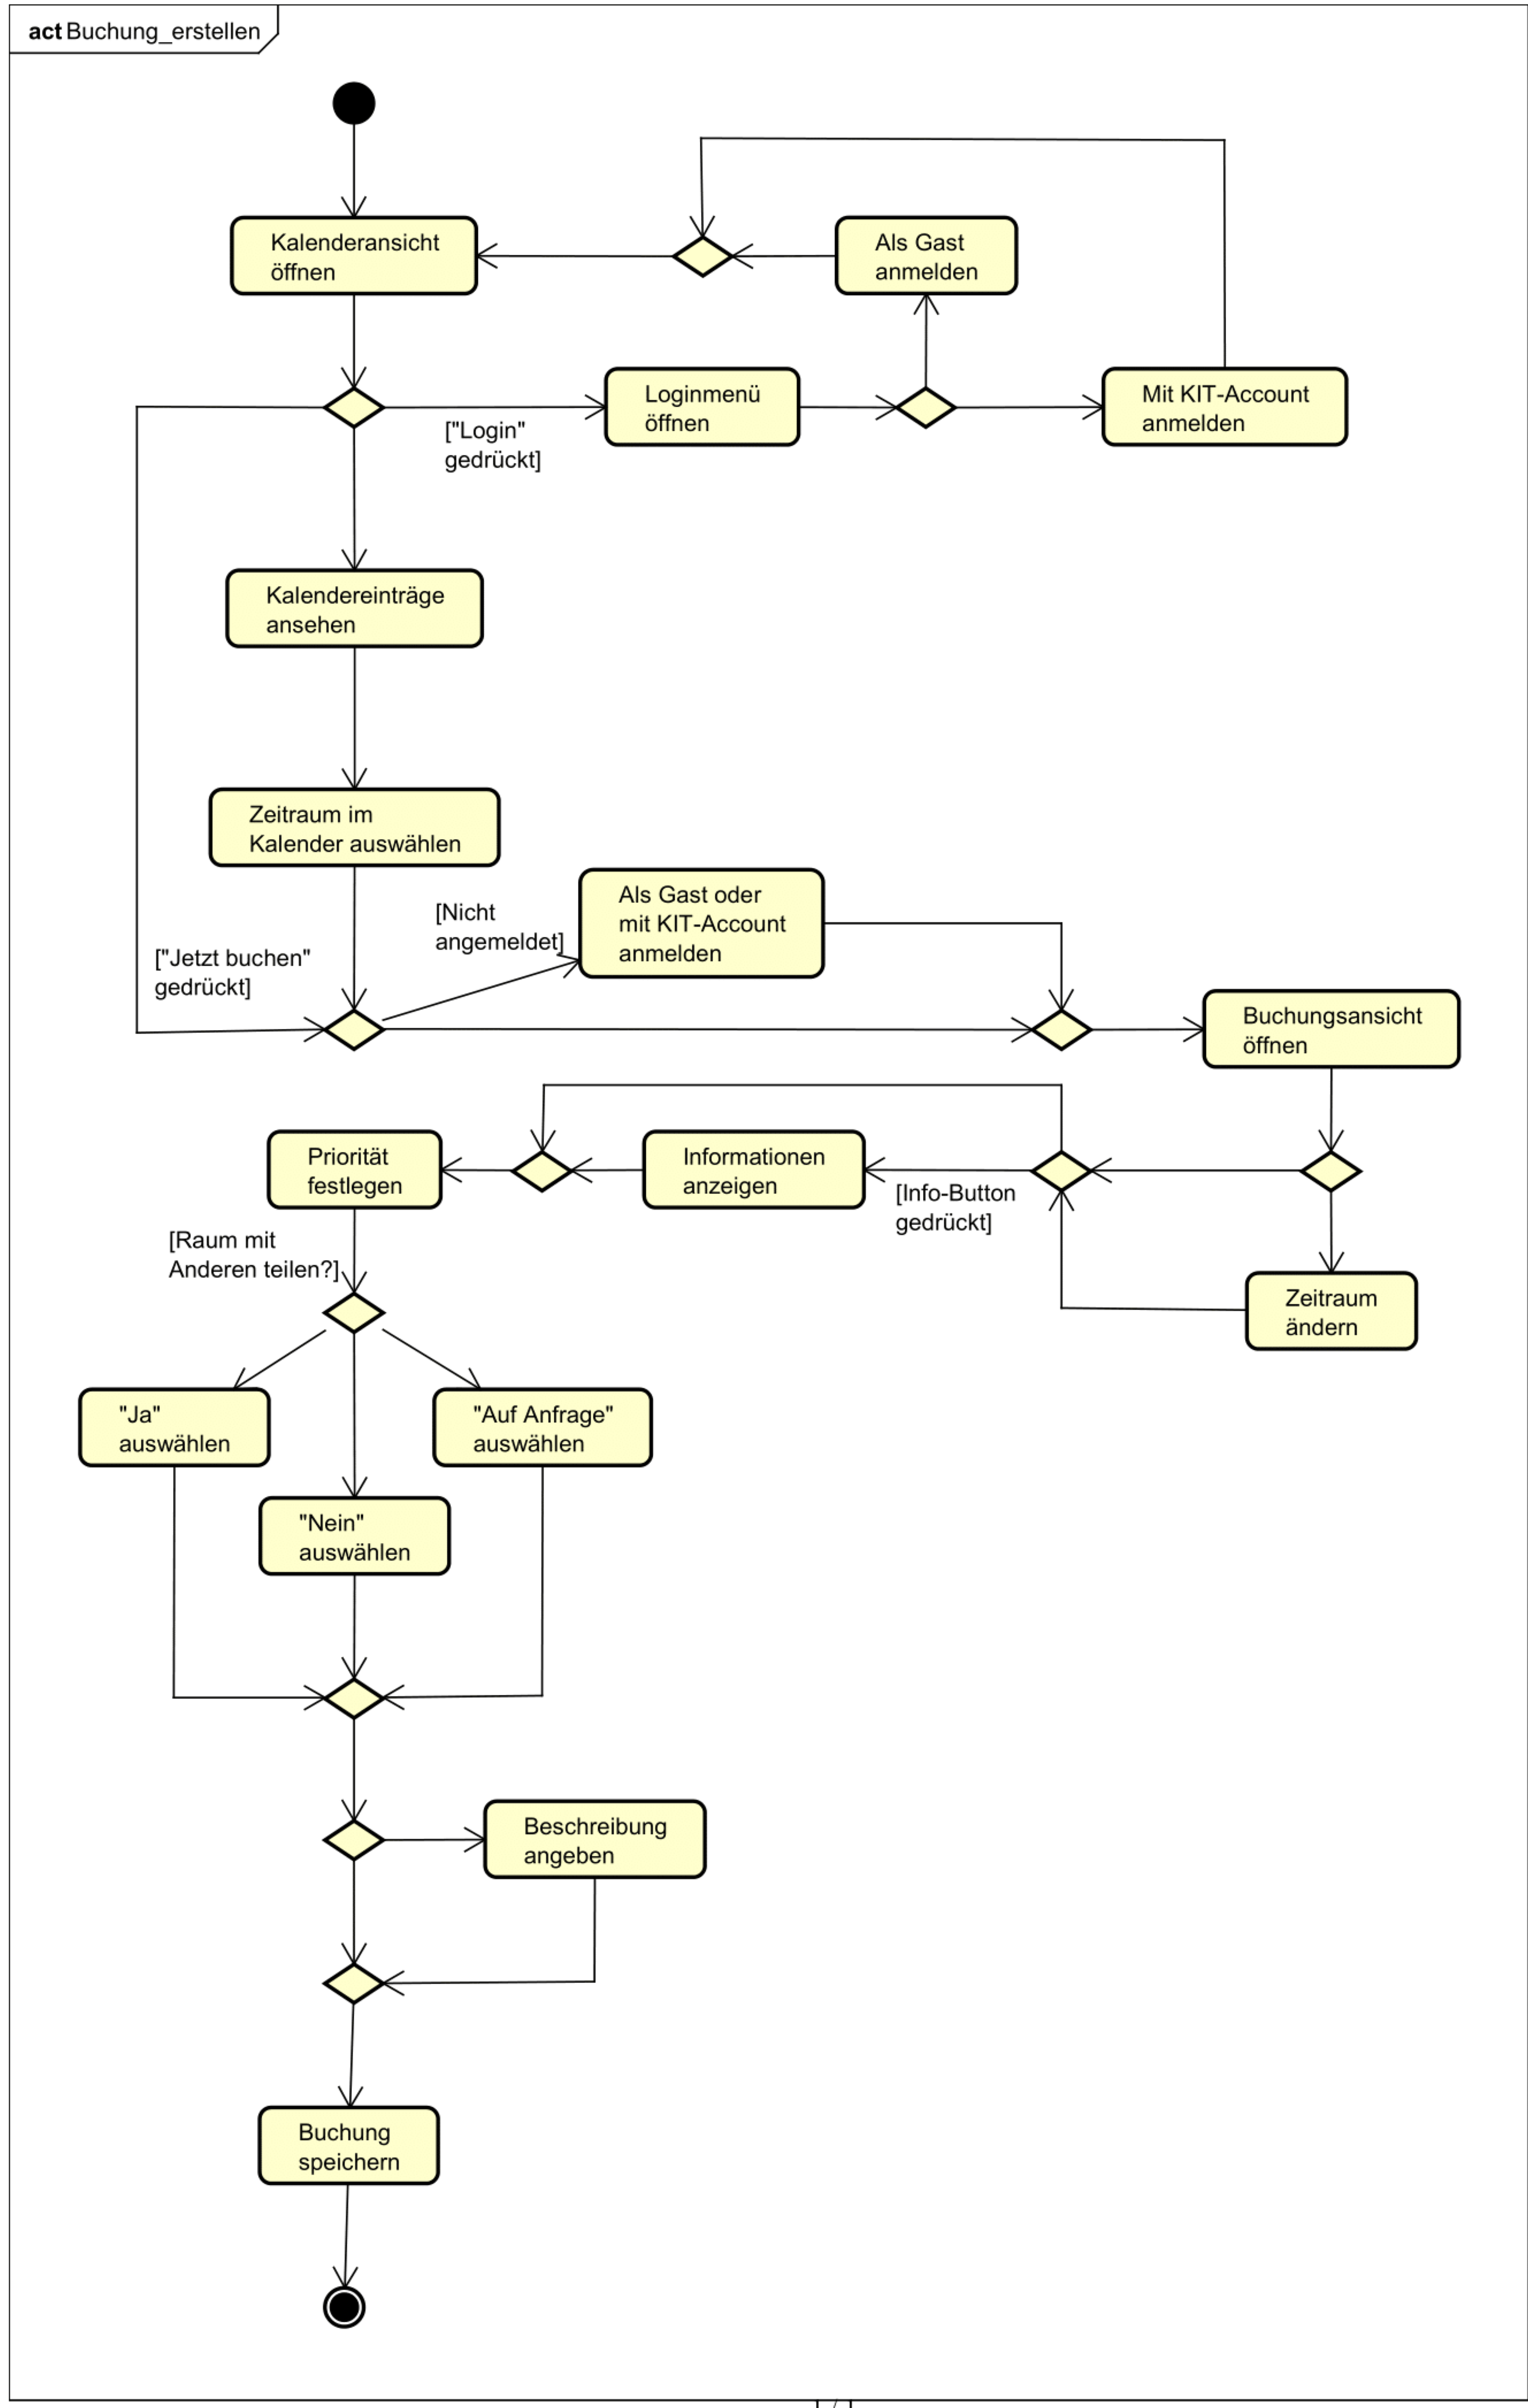
\includegraphics[width=\textwidth]{figures/activity/buchungerstellen}
    \caption{Diagramm zur Erklärung des Buchungserstellungsprozesses}
    \label{fig:make-booking-diagram}
\end{figure}

Dieses Sequenzdiagramm zeigt den Ablauf der Buchungserstellung auf der Programmebene.

\begin{figure}[ht]
    \centering
    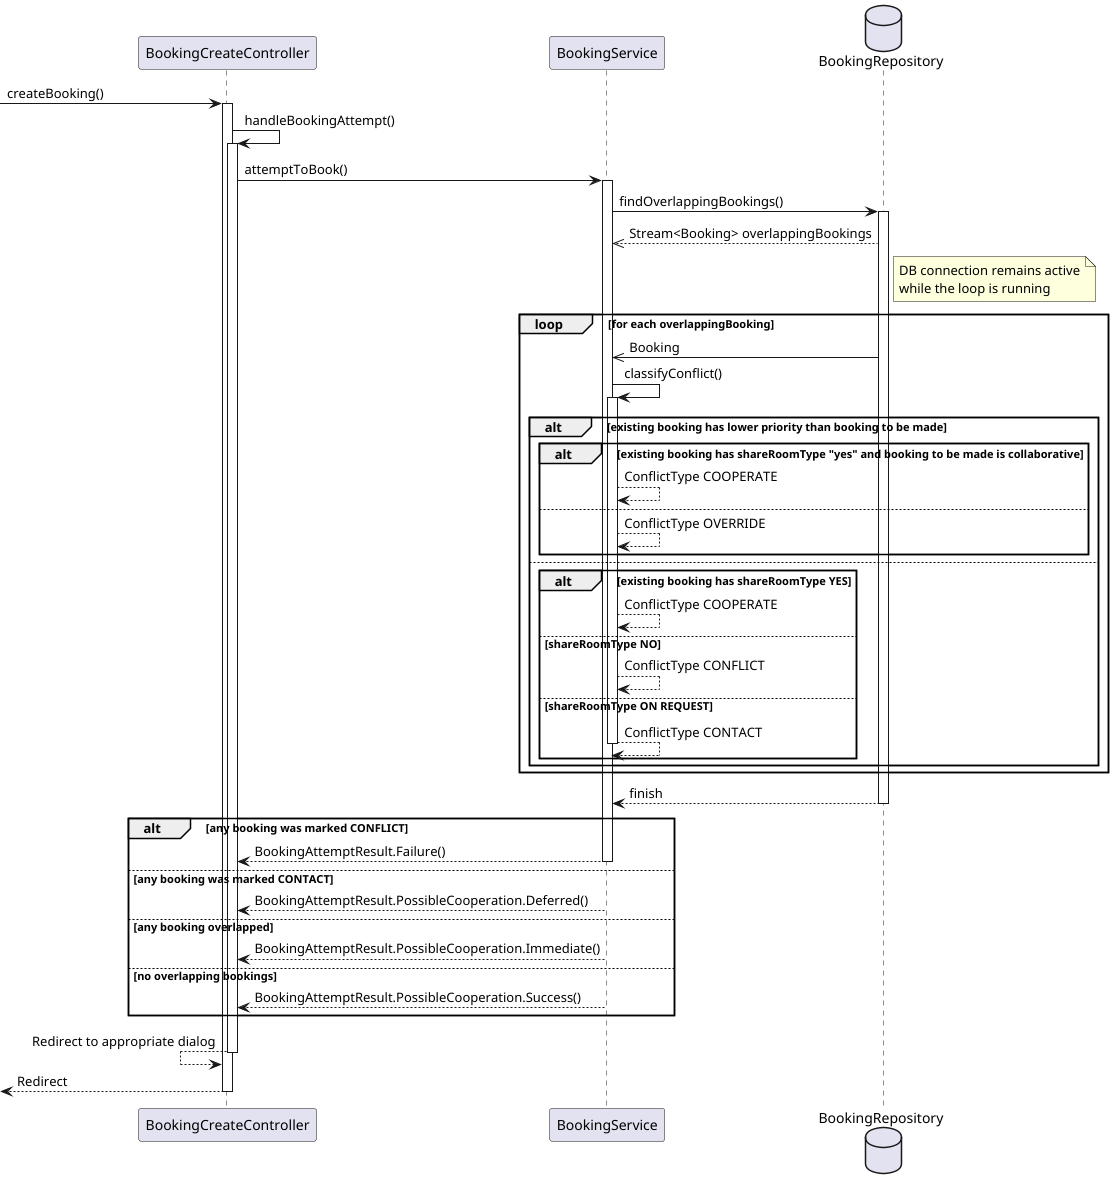
\includegraphics[width=\textwidth]{figures/activity/SequenzdiagrammBuchungErstellen}
    \caption{Sequenzdiagramm zur Erklärung des Buchungserstellungsprozesses}
    \label{fig:make-booking-sequence-diagram}

\subsection{Konfliktlösung bei Buchungserstellung}

Bei der Erstellung eines Termins kann ein Terminkonflikt auftreten, falls im angegebenen Zeitraum bereits eine
Buchung getätigt wurde. In diesem Fall wird nach der Priorität der Buchung entschieden und die Buchung mit
höherer Priorität wird beibehalten. Im Fall, dass beide Buchungen die gleiche Priorität haben, wird die zuerst
erstellte Buchung beibehalten. Wenn beide Buchungen bei der Kategorie "Raum teilen" auf "Ja" gesetzt sind, wird die
Buchung mit der niedrigeren Priorität beibehalten. Falls die zuerst getätigte Buchunge auf "Auf Anfrage" steht,
besteht die Möglichkeit eine Anfrage zu stellen.

Das Ablaufdiagramm stellt den oben beschrieben Konliktlösungsprozess dar.

\begin{figure}[ht]
    \centering
    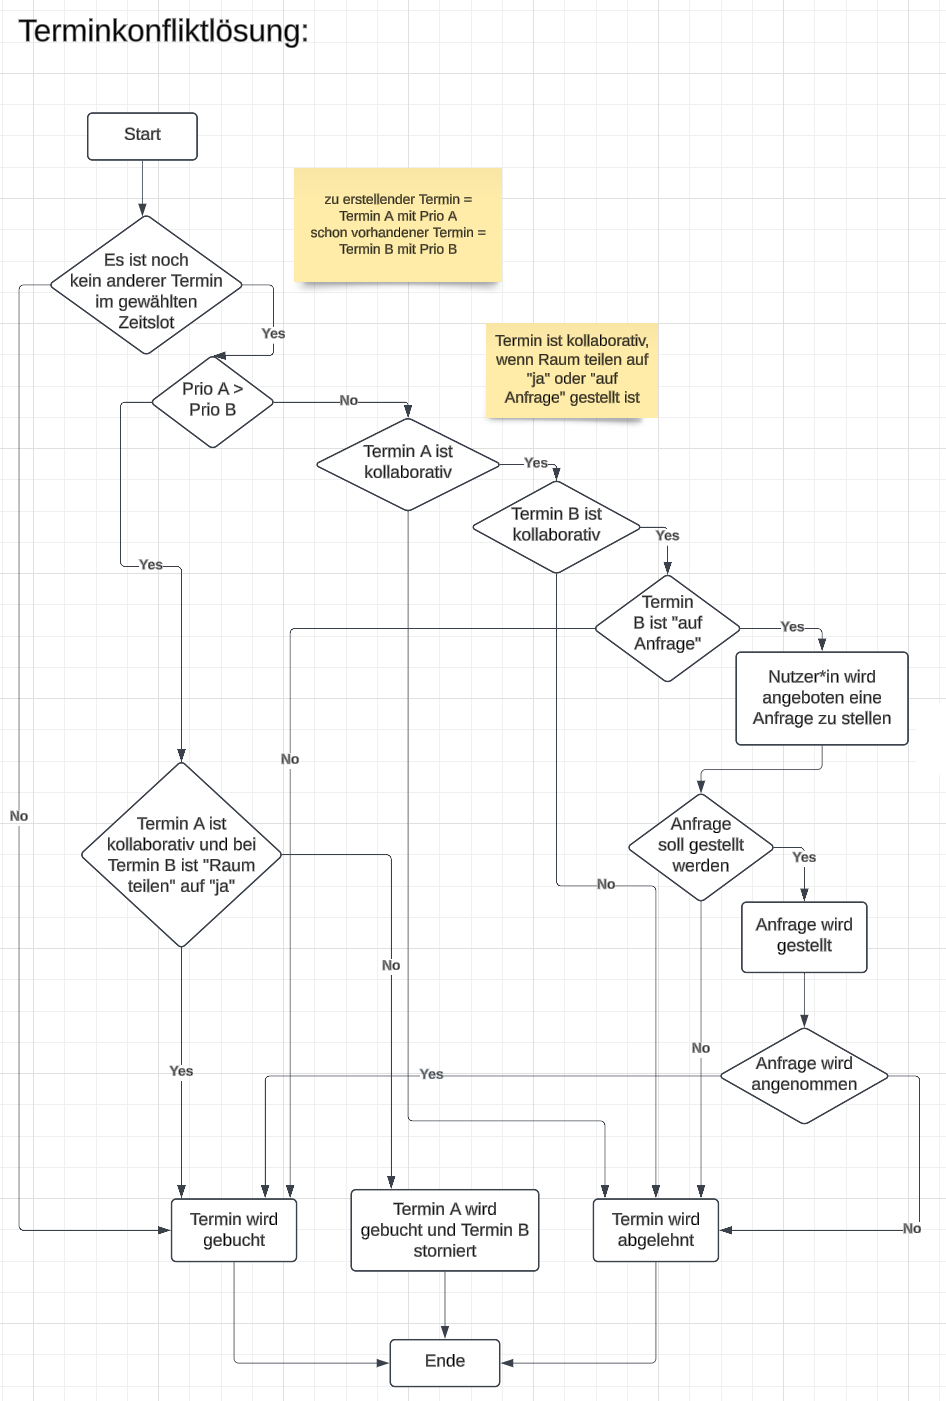
\includegraphics[width=\textwidth]{figures/activity/terminkonfliktloesung}
    \caption{Diagramm zur Erklärung des Konfliktlösungsprozesses bei der Buchungserstellung}
    \label{fig:resolve-conflict-diagram}
\end{figure}
\clearpage

\section{Buchungen Verwalten}

Die Website bietet die Möglichkeit, die eigenen Buchungen zu verwalten. Mit der Voraussetzung,
dass man angemeldet ist, kann man die Terminübersicht, welche eine Liste der eigenen Termine anzeigt,
öffnen und hat dann die Möglichkeit Termine zu löschen.

Das Ablaufdiagramm beschreibt den Ablauf des Buchungsverwaltungsprozesses.

\begin{figure}[ht]
    \centering
    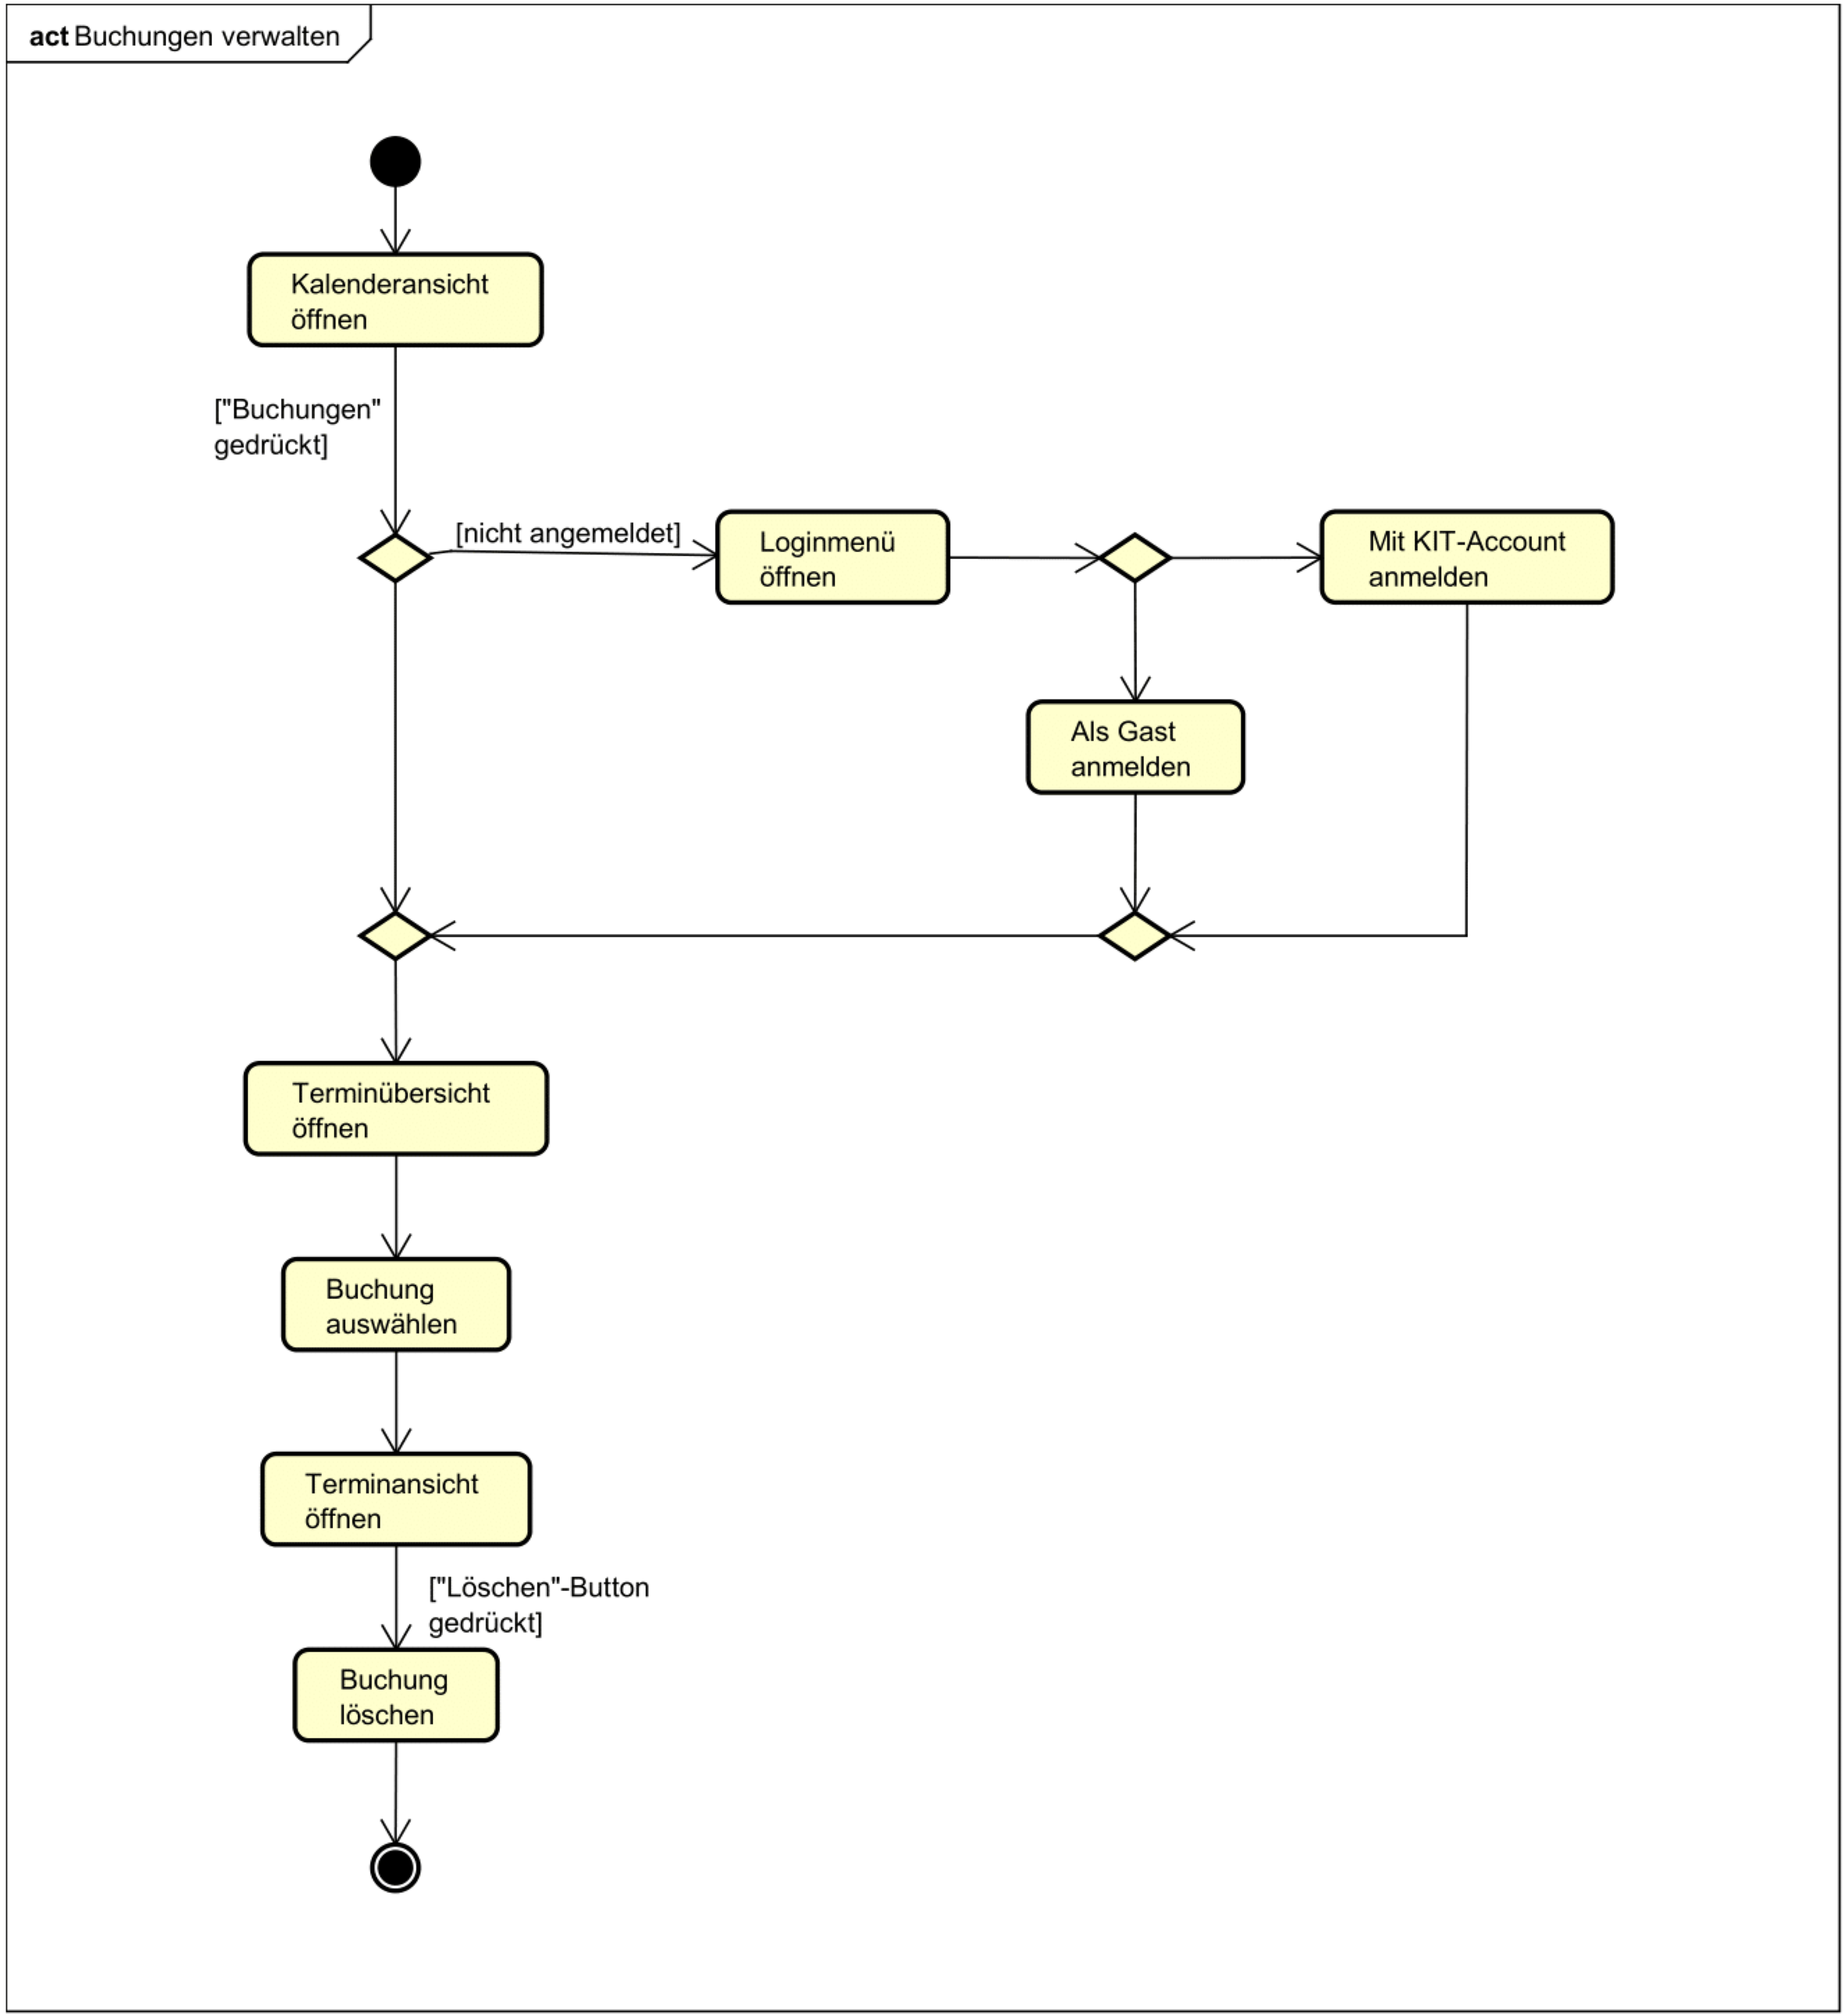
\includegraphics[width=\textwidth]{figures/activity/buchungverwalten}
    \caption{Diagramm zur Erklärung des Buchungsverwaltungsprozesses}
    \label{fig:manage-booking-diagram}
\end{figure}
\clearpage

\section{Terminaktionen}

Hier wird die Funktionalität der Terminansicht dargestellt. Wenn der angesehene Termin ein eigener Termin ist
oder man als Admin eingeloggt ist, gibt es hier die Möglichkeit den gewählten Termin zu löschen. Ist der
Termin nicht der eigene und er steht auf "auf Anfrage" teilen, dann gibt es einen Anfrage-Button über diesen man
eine Anfrage schicken kann.

\begin{figure}[ht]
    \centering
    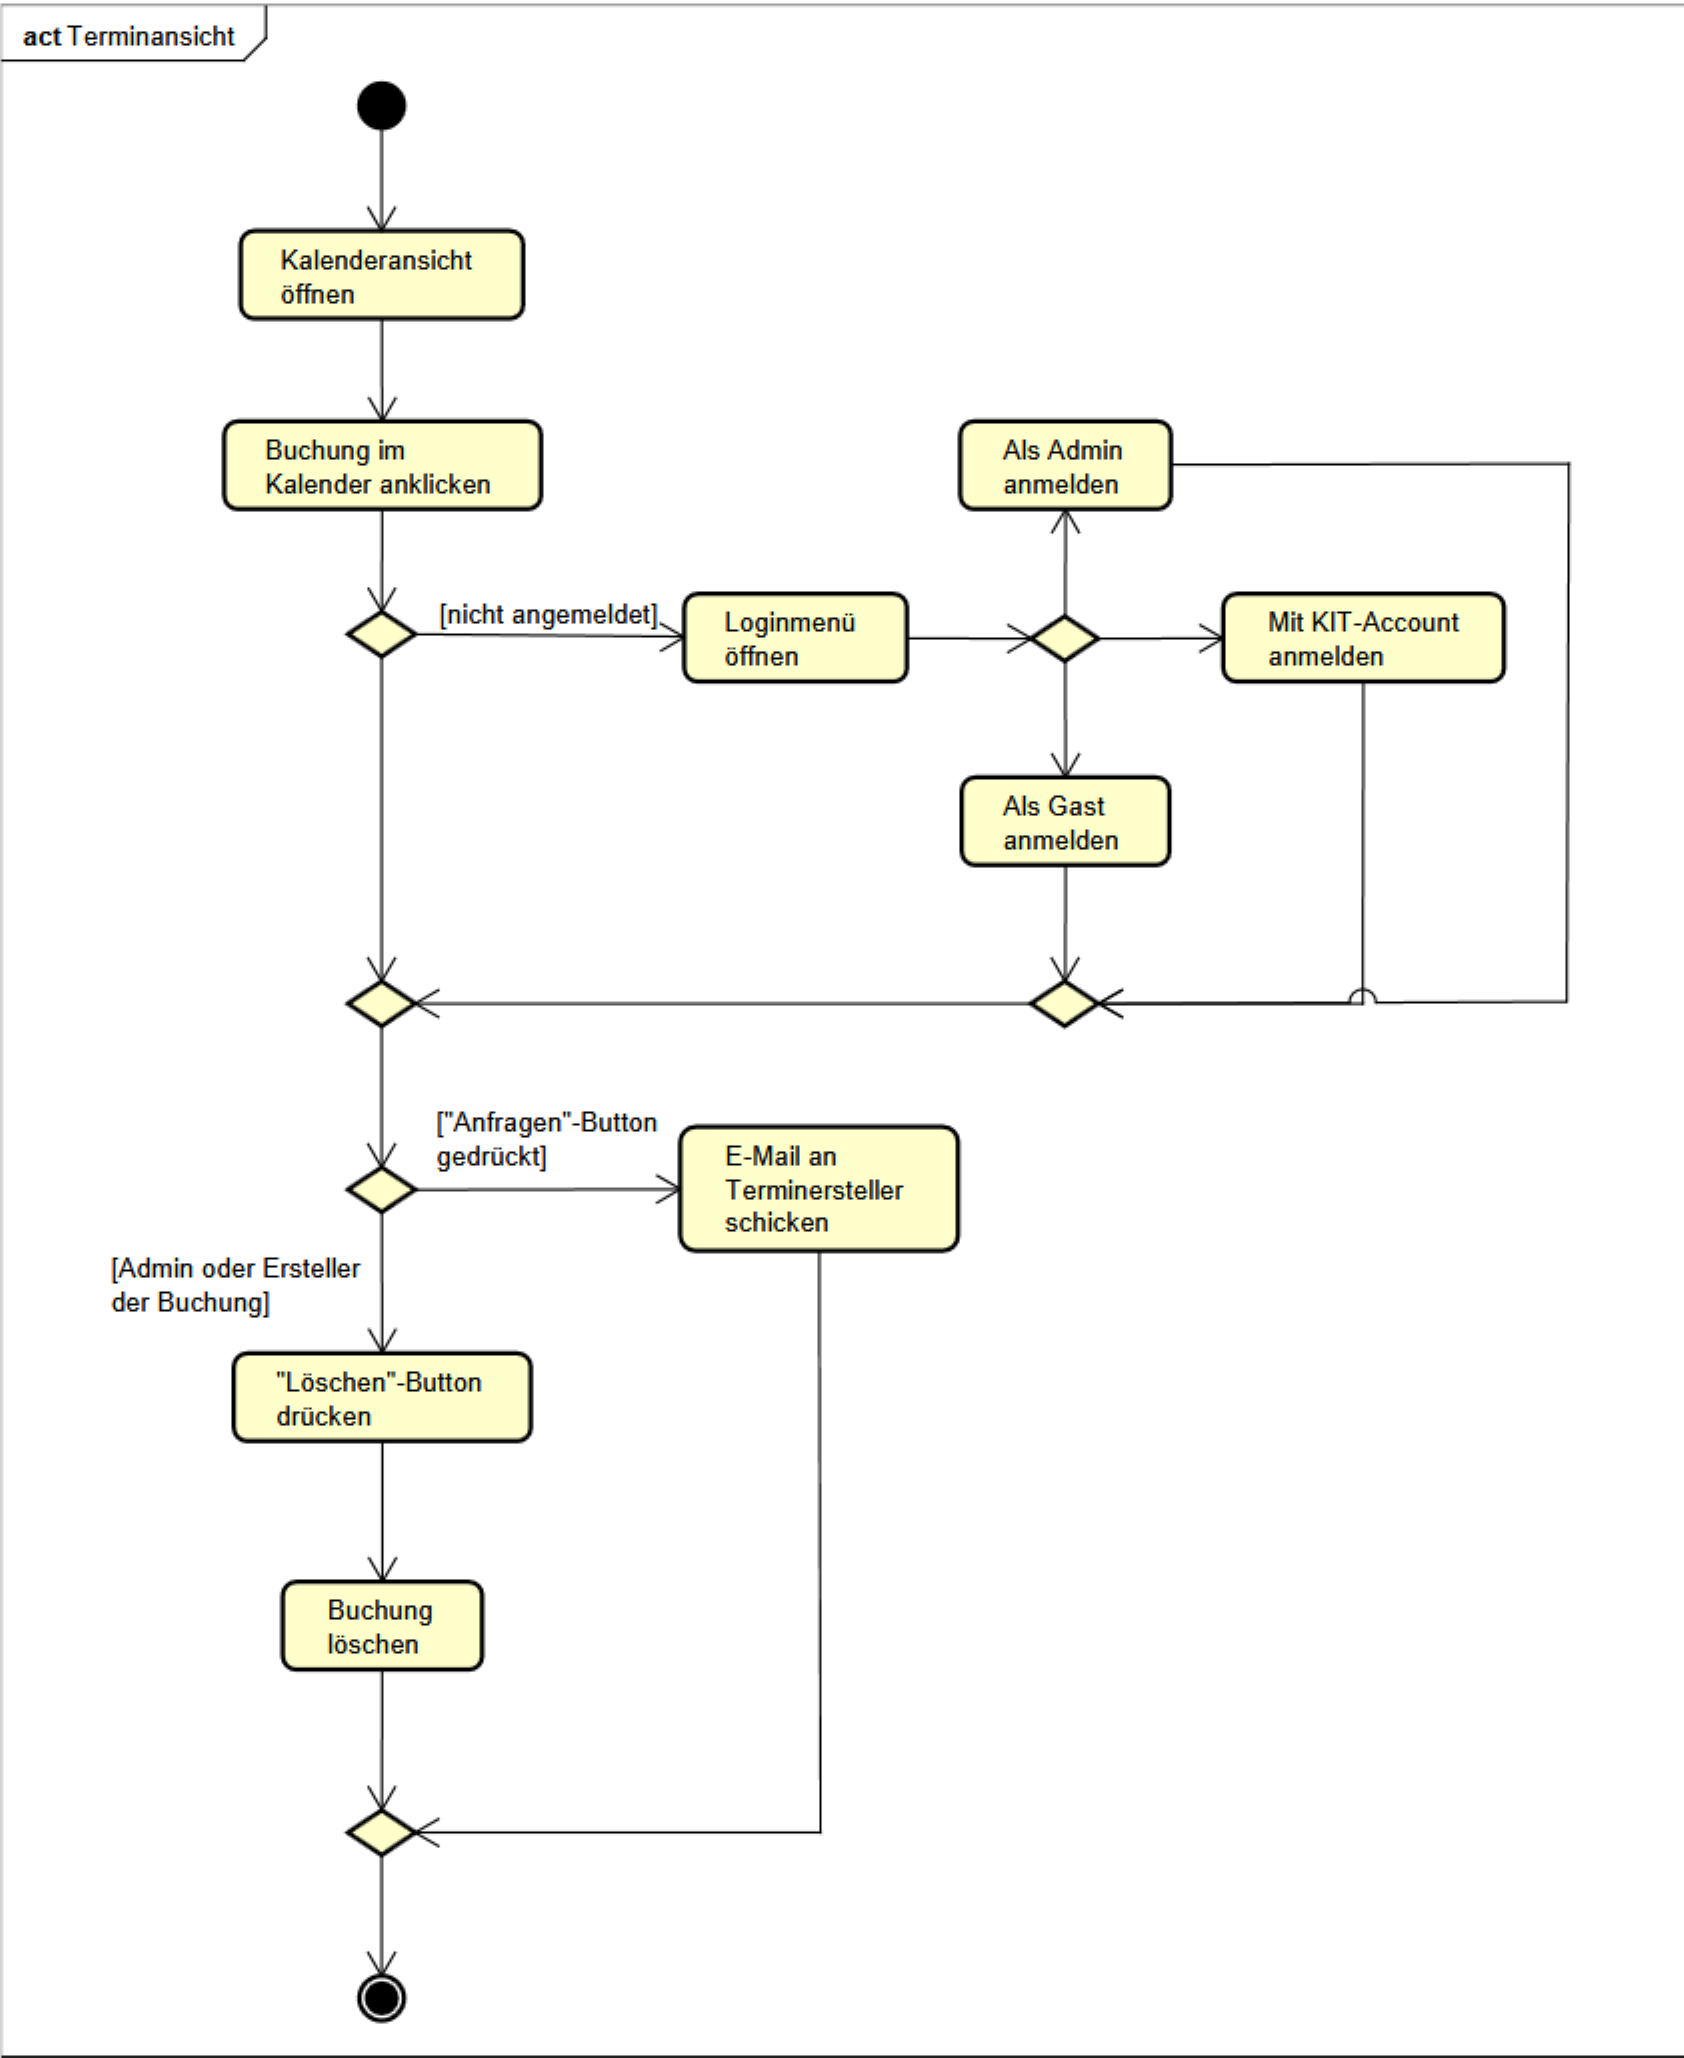
\includegraphics[width=\textwidth]{figures/activity/terminansicht}
    \caption{Diagramm zur Erklärung der Terminaktionen}
    \label{fig:booking-actions-diagram}
\end{figure}
\clearpage

\section{Checkoutprozess}

Der Checkout-Button bietet die Möglichkeit die eigene laufende Buchung vorzeitig zu beenden und den Raum für andere Nutzende freizugeben.

\begin{figure}[ht]
    \centering
    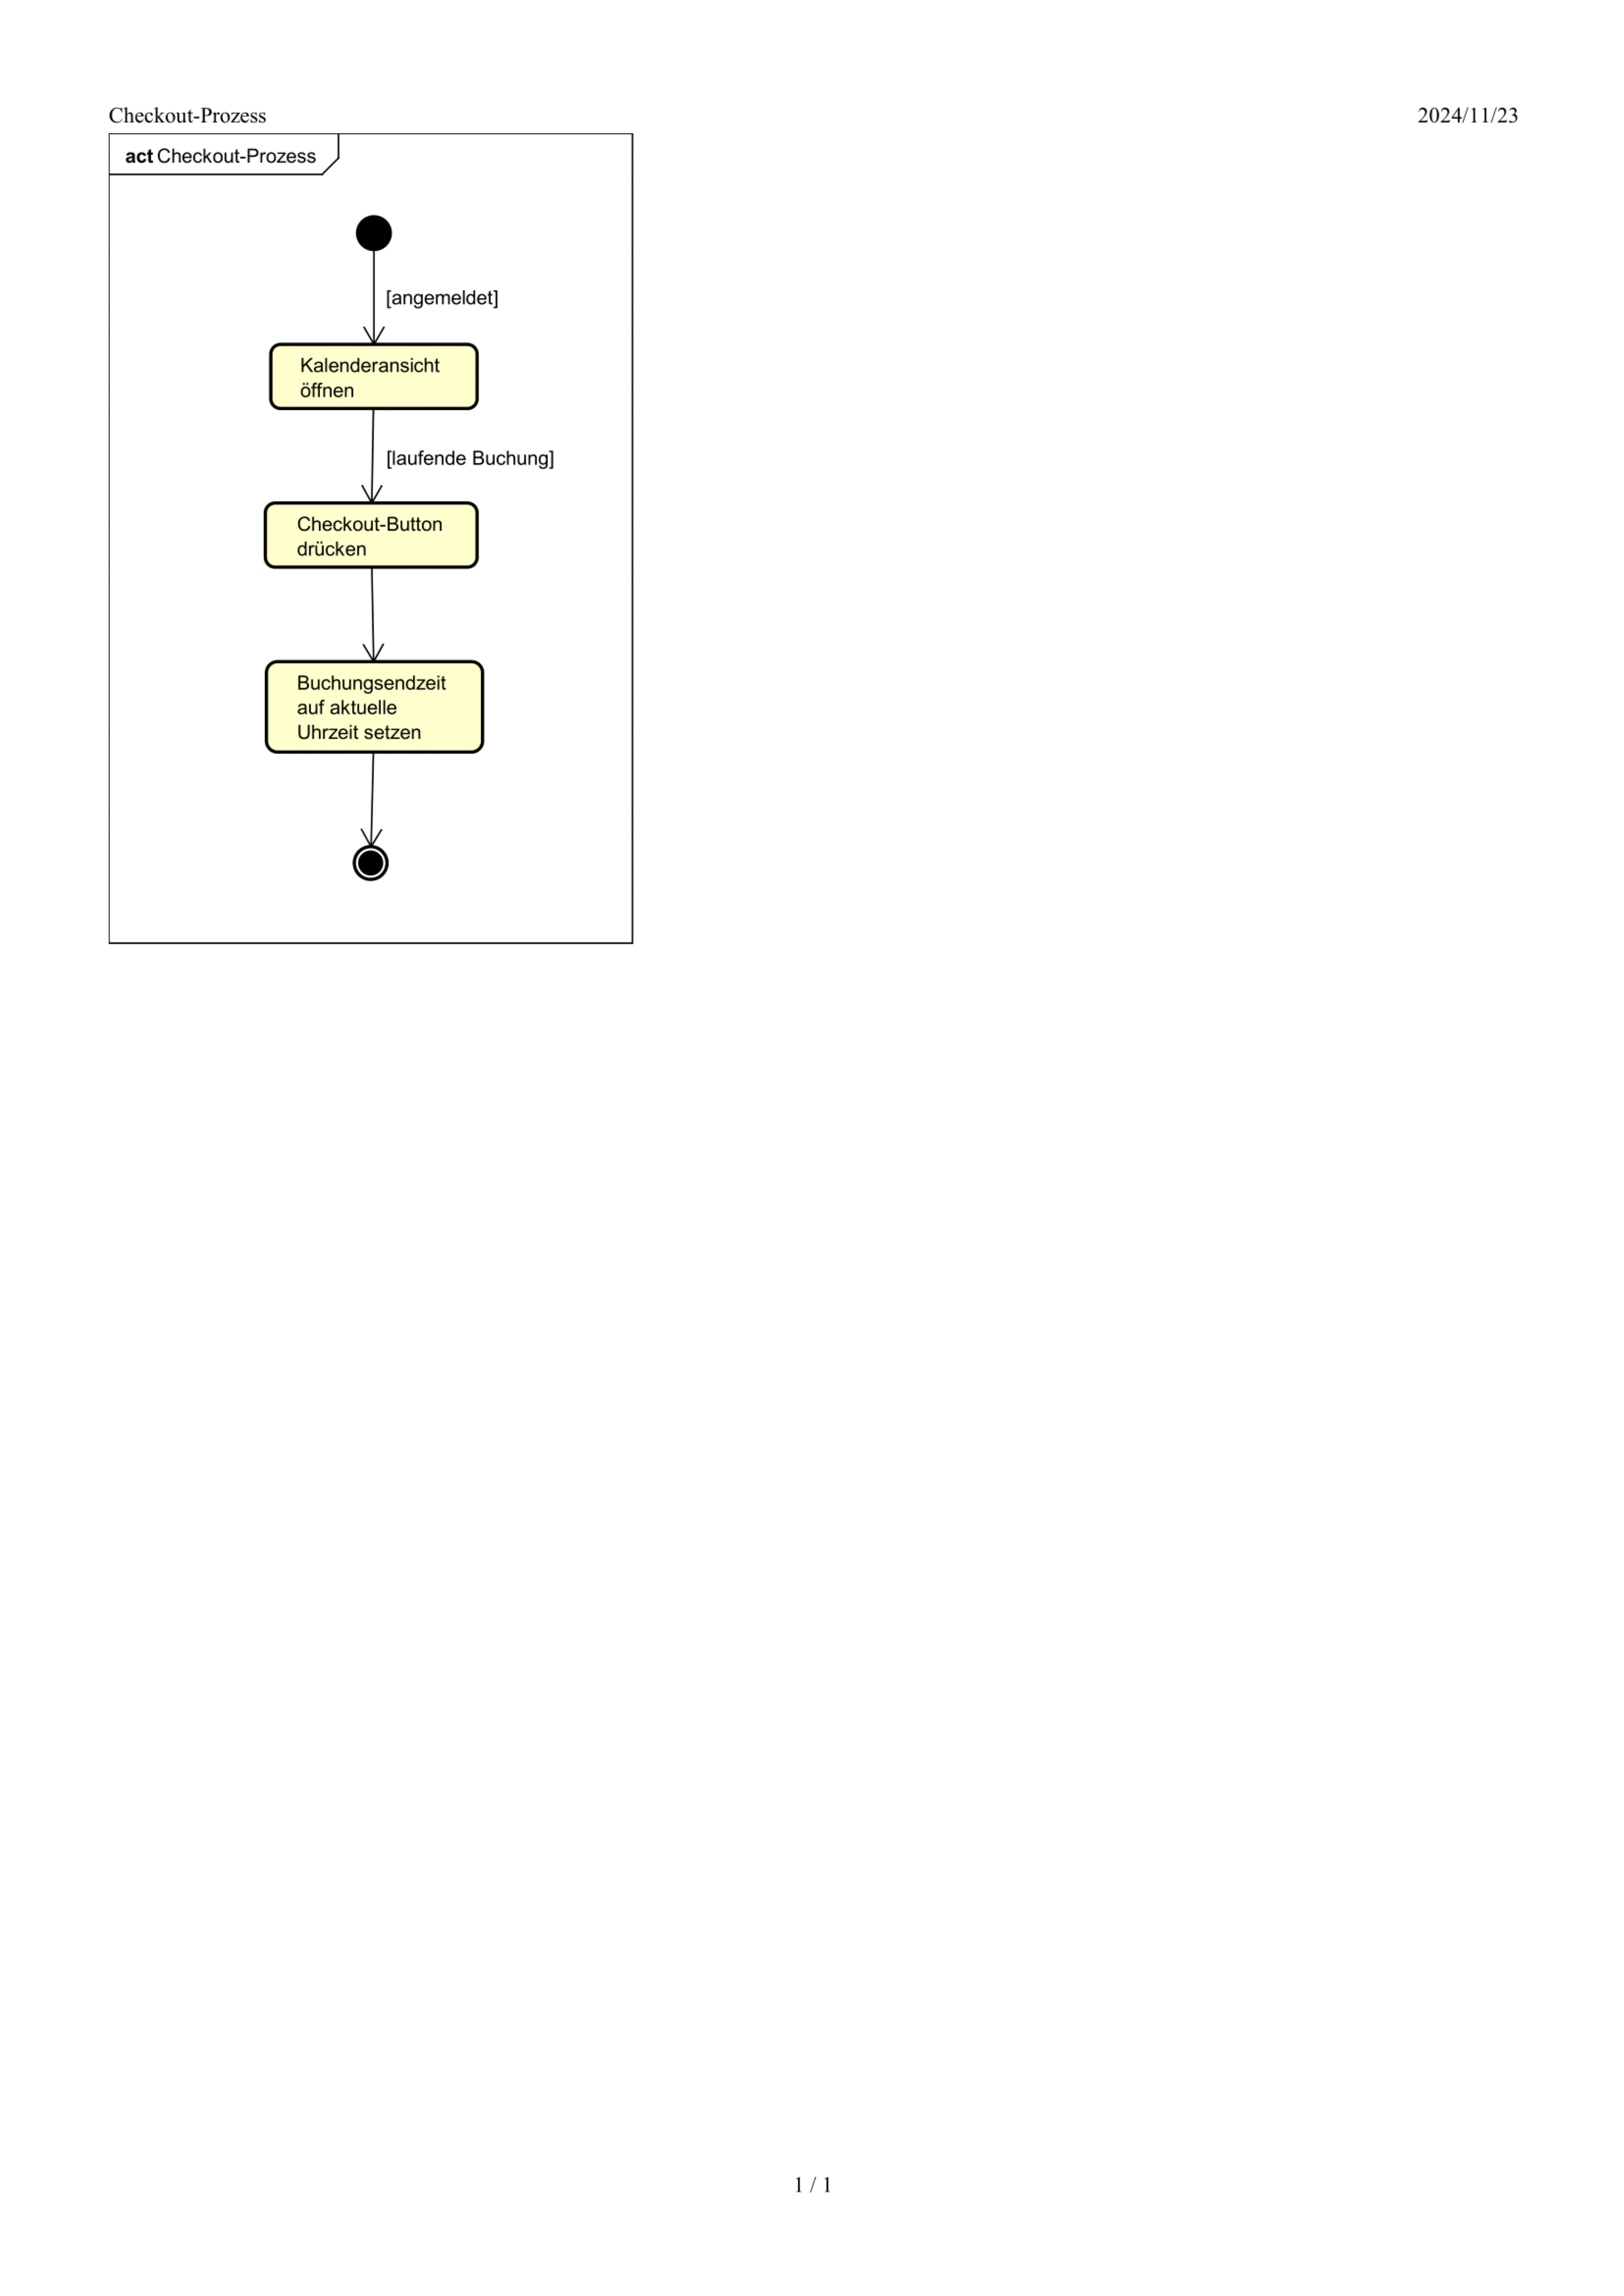
\includegraphics[width=\textwidth]{figures/activity/checkoutprozess}
    \caption{Diagramm zur Erklärung des Abmeldeprozesses}
    \label{fig:logout-diagram}
\end{figure}

\clearpage

\section{Adminfunktionalität}

Die Adminfunktionalität beinhaltet mehrere Möglichkeiten, die Website zu verwalten.
Es kann ein Termin gelöscht, Kontos gebannt, die Öffnungszeiten geändert und die Gästefunktion
ausgeschalten werden.

Dieses Ablaufdiagramm stellt die unterschiedlichen Aktionsmöglichkeiten des/r Admins dar.

\begin{figure}[ht]
    \centering
    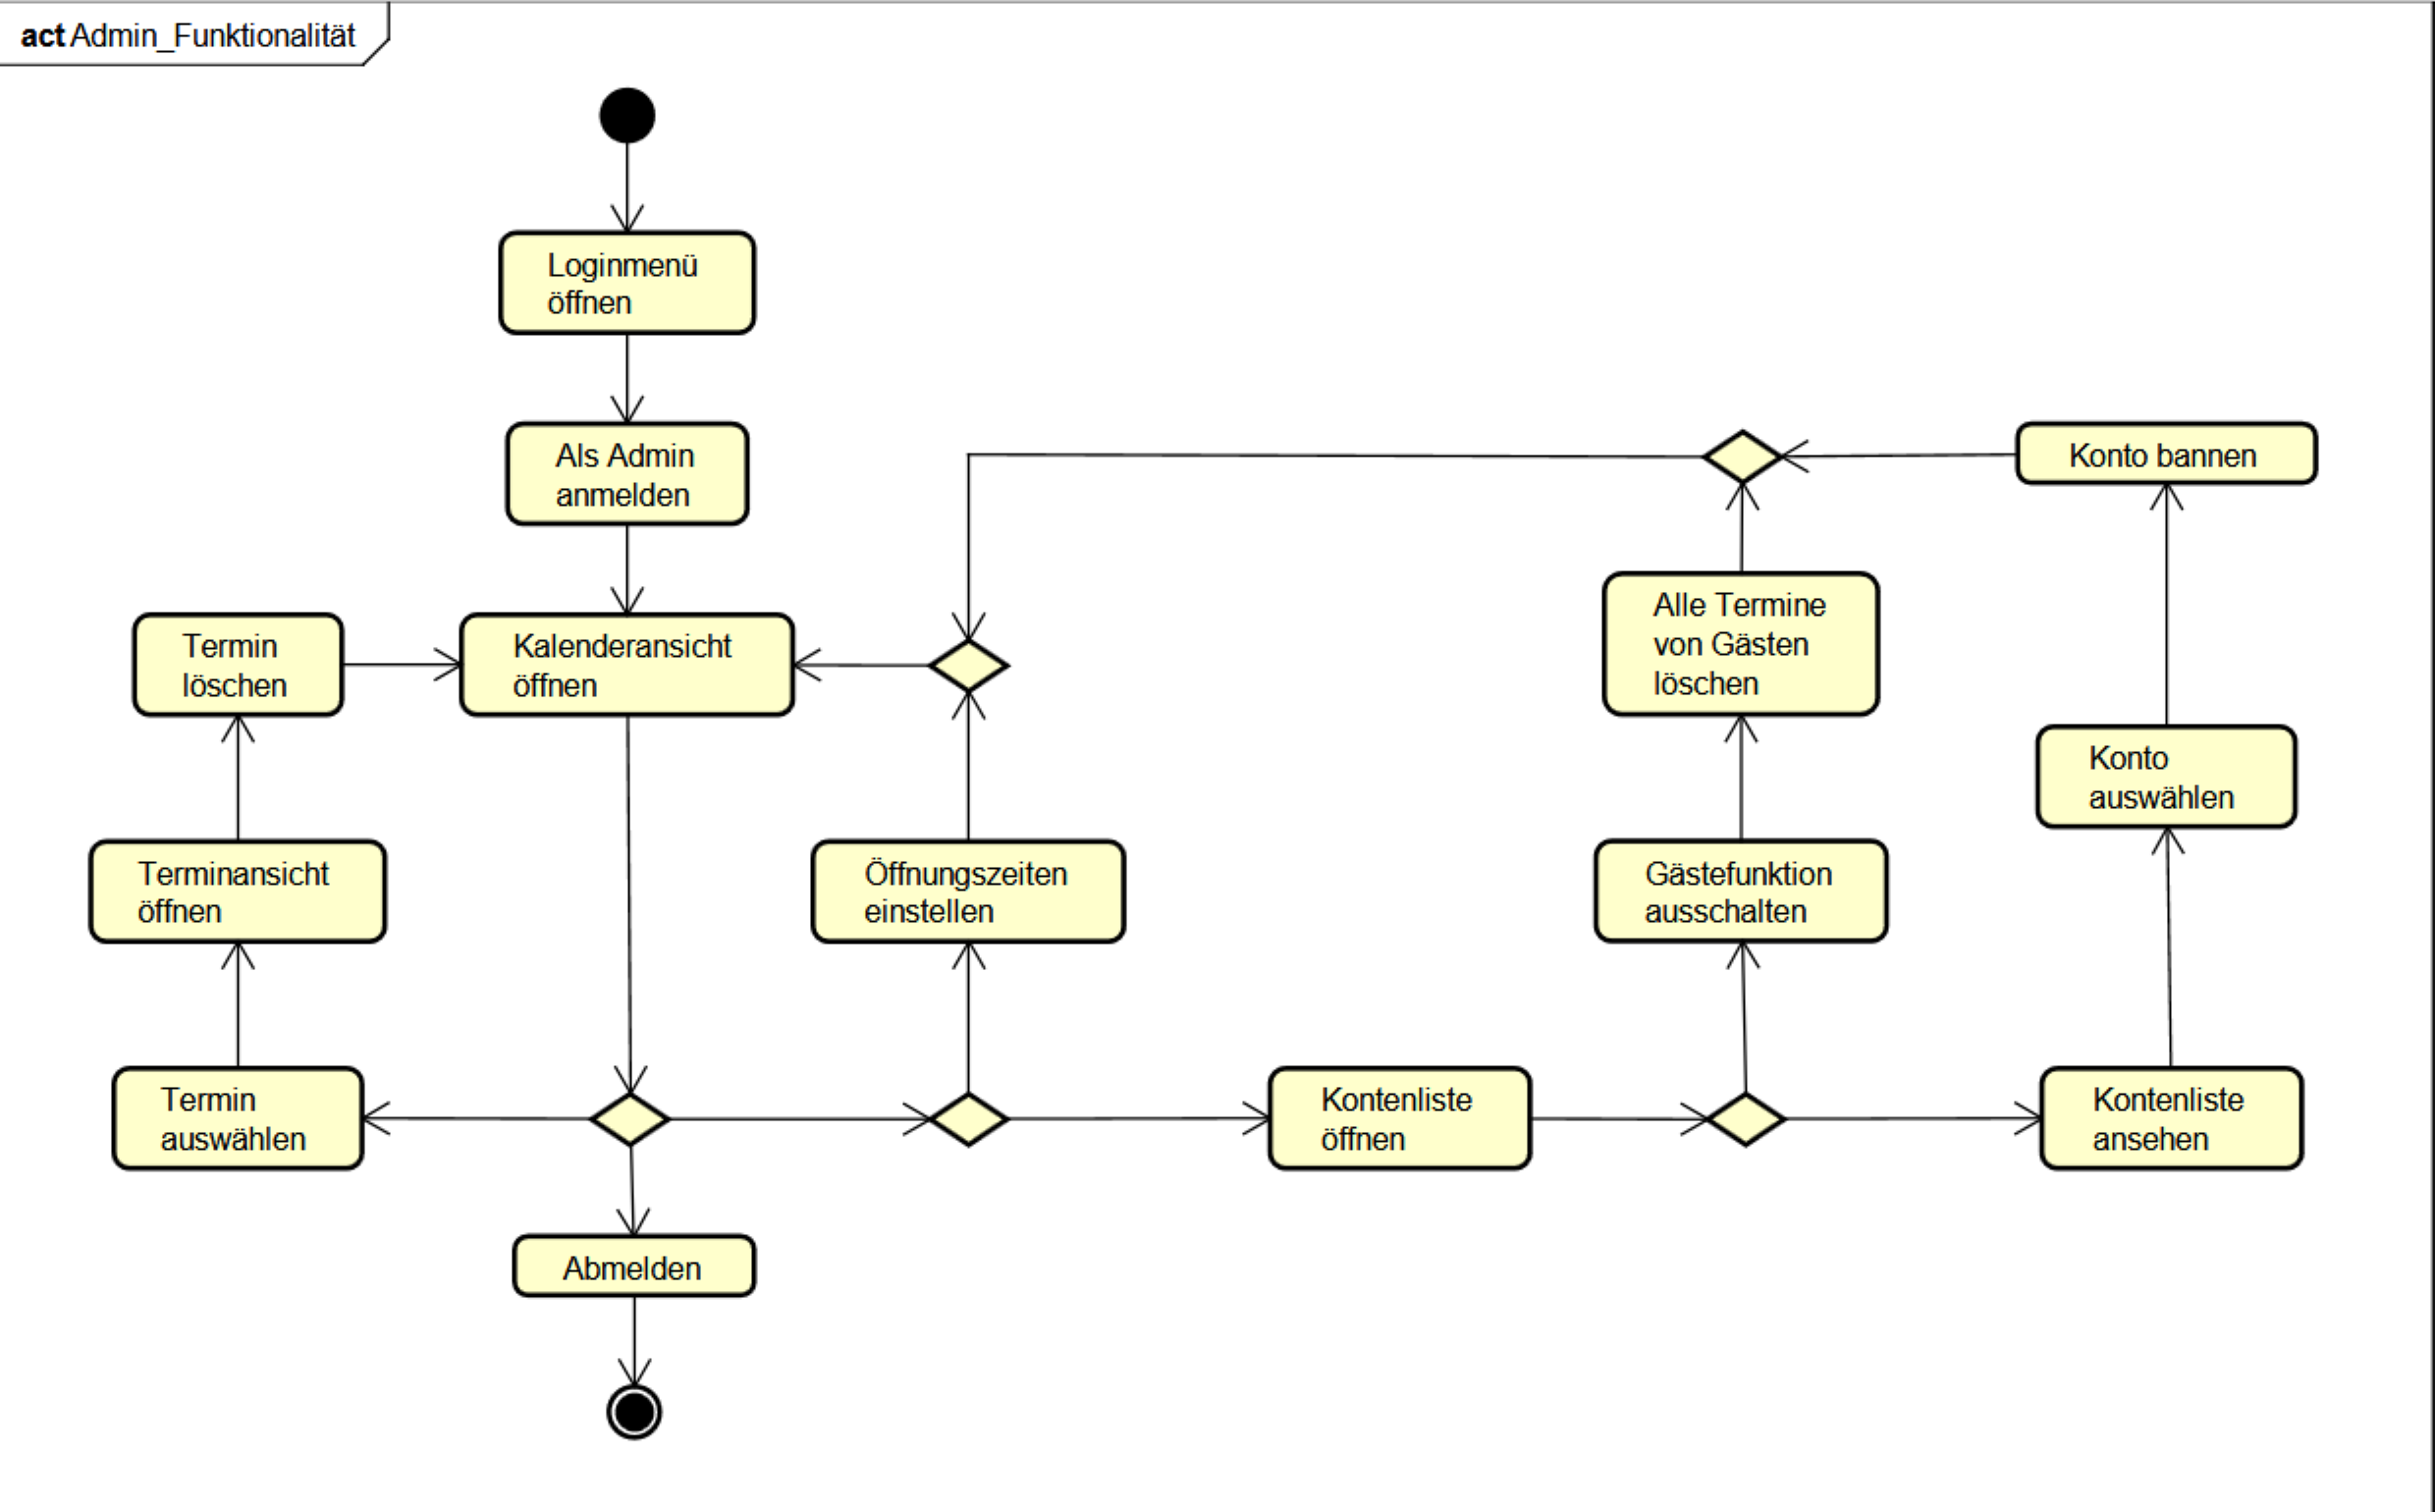
\includegraphics[width=\textwidth]{figures/activity/adminfunk}
    \caption{Diagramm zur Erklärung der Adminfunktionalität}
    \label{fig:admin-functions-diagram}
\end{figure}
\clearpage

      
% Dazu jeweils Tests

\printglossaries

%------Ende des Dokumentes------------------------------------------------------
\end{document}
